\documentclass{article}
\usepackage[utf8]{inputenc}
\usepackage{amsmath}
\usepackage{graphicx}
\usepackage{amsfonts}
\usepackage{algorithm}
\usepackage{algorithmic}
\usepackage{adjustbox}
\usepackage{listings}
\usepackage{color}
\usepackage{algpseudocode}
\graphicspath{{/home/soham/Desktop/NEAlatex/images/}}
\definecolor{dkgreen}{rgb}{0,0.6,0}
\definecolor{gray}{rgb}{0.5,0.5,0.5}
\definecolor{mauve}{rgb}{0.58,0,0.82}

\lstset{frame=tb,
  language=Python,
  aboveskip=3mm,
  belowskip=3mm,
  showstringspaces=false,
  columns=flexible,
  basicstyle={\small\ttfamily},
  numbers=none,
  numberstyle=\tiny\color{gray},
  keywordstyle=\color{blue},
  commentstyle=\color{dkgreen},
  stringstyle=\color{mauve},
  breaklines=true,
  breakatwhitespace=true,
  tabsize=3
}
\title{Deep Stock Prediction}

\author{Soham Deshpande}
\date{January 2022}

\begin{document}

\maketitle
\subsection*{A Technical Indicator for  liquid asset evaluation using machine learning techniques }
\clearpage
\tableofcontents

\clearpage

\section {Introduction to the Stock Market}
\subsection{Abstract}
\normalsize{In recent years the fast-growing financial markets opened new horizons for investors and at the same time brought new challenges for financial analysts in their efforts to make effective decisions and reduce investment risks.
The stock market is a highly dynamic and complex system where factors affecting the price are not limited to the economic world, rather in recent years the political climate and social media playing a bigger role. This has resulted in a highly stochastic, chaotic market. As with the other industries, the amount of data being created every day can be overwhelming and often hard to understand and decipher for someone with limited experience. This problem can be seen as one for computer science and mathematics.
In the past decades, effective prediction models, both linear and machine learning tools have been explored. In recent years the research into deep learning has rapidly accelerated the progress made in prediction software. The motivation behind this paper is to describe and show an implementation of a deep learning model to help predict the price of stocks.
\\
Keywords:
Stock market prediction, deep learning, transformers, attention, feedforward neural network, temporal fusion transformers
}

\section{Introduction}
The model I will be exploring is a transformer-based deep learning architecture that takes advantage of attention, more specifically multi-head attention in my implementation.
Many models use ARIMA(Auto-Regressive Integrated Moving Average) but I am proposing using transformers with multi-head attention, something that I will talk about later on, to help the model ‘learn’ about the stock rather than just trying to fit a curve on it based on the last few data points. The benefits of learning allow the model to consider previous experience instead of just looking at a few, previous data points. This technique will hopefully result in a higher accuracy compared to ARIMA. Other implementations have managed an accuracy of 94\%(Zolkepli and Divino, n.d.) so I will be aiming to stay within 5\%. The reduced target comes down to a few factors such as limited access hardware, not enough time to optimise my program for the hardware as well as a few other factors.



\section{Analysis}
\subsection{Stock prediction techniques}
Stock prediction is a problem that requires time series analysis. Time series analysis is the technique of analysing sequential data.
In the current market, a couple of techniques are used to analyse and predict the price. In this section, I will discuss a few multivariate time series models.

\subsection{ARIMA}
Autoregressive integrated moving average is a common method used to perform time series analysis.
(Hyndman and Athanasopoulos, 2018)
In a regression model, we forecast the variable of interest using a linear combination of predictors. Autoregression focuses on using a linear combination of past values and the variable itself to predict the variable of interest. The term autoregression indicates that it is a regression of the variable against itself.

\begin{equation}
    y_t = c + \phi_1 y_{t-1} + \phi_2 {t-2} + ... + \phi_p y_{t-p} + \epsilon_t
\end{equation}

These models are very good at handling different time series patterns. Changing the parameters, $\phi$ result in different patterns. $\epsilon$ is the error term; changing this will change the scale of the series. This model is very effective when it comes to stock prediction and so will therefore provide a baseline when it comes to the accuracy of the model.
\begin{figure}[h]
    \centering
    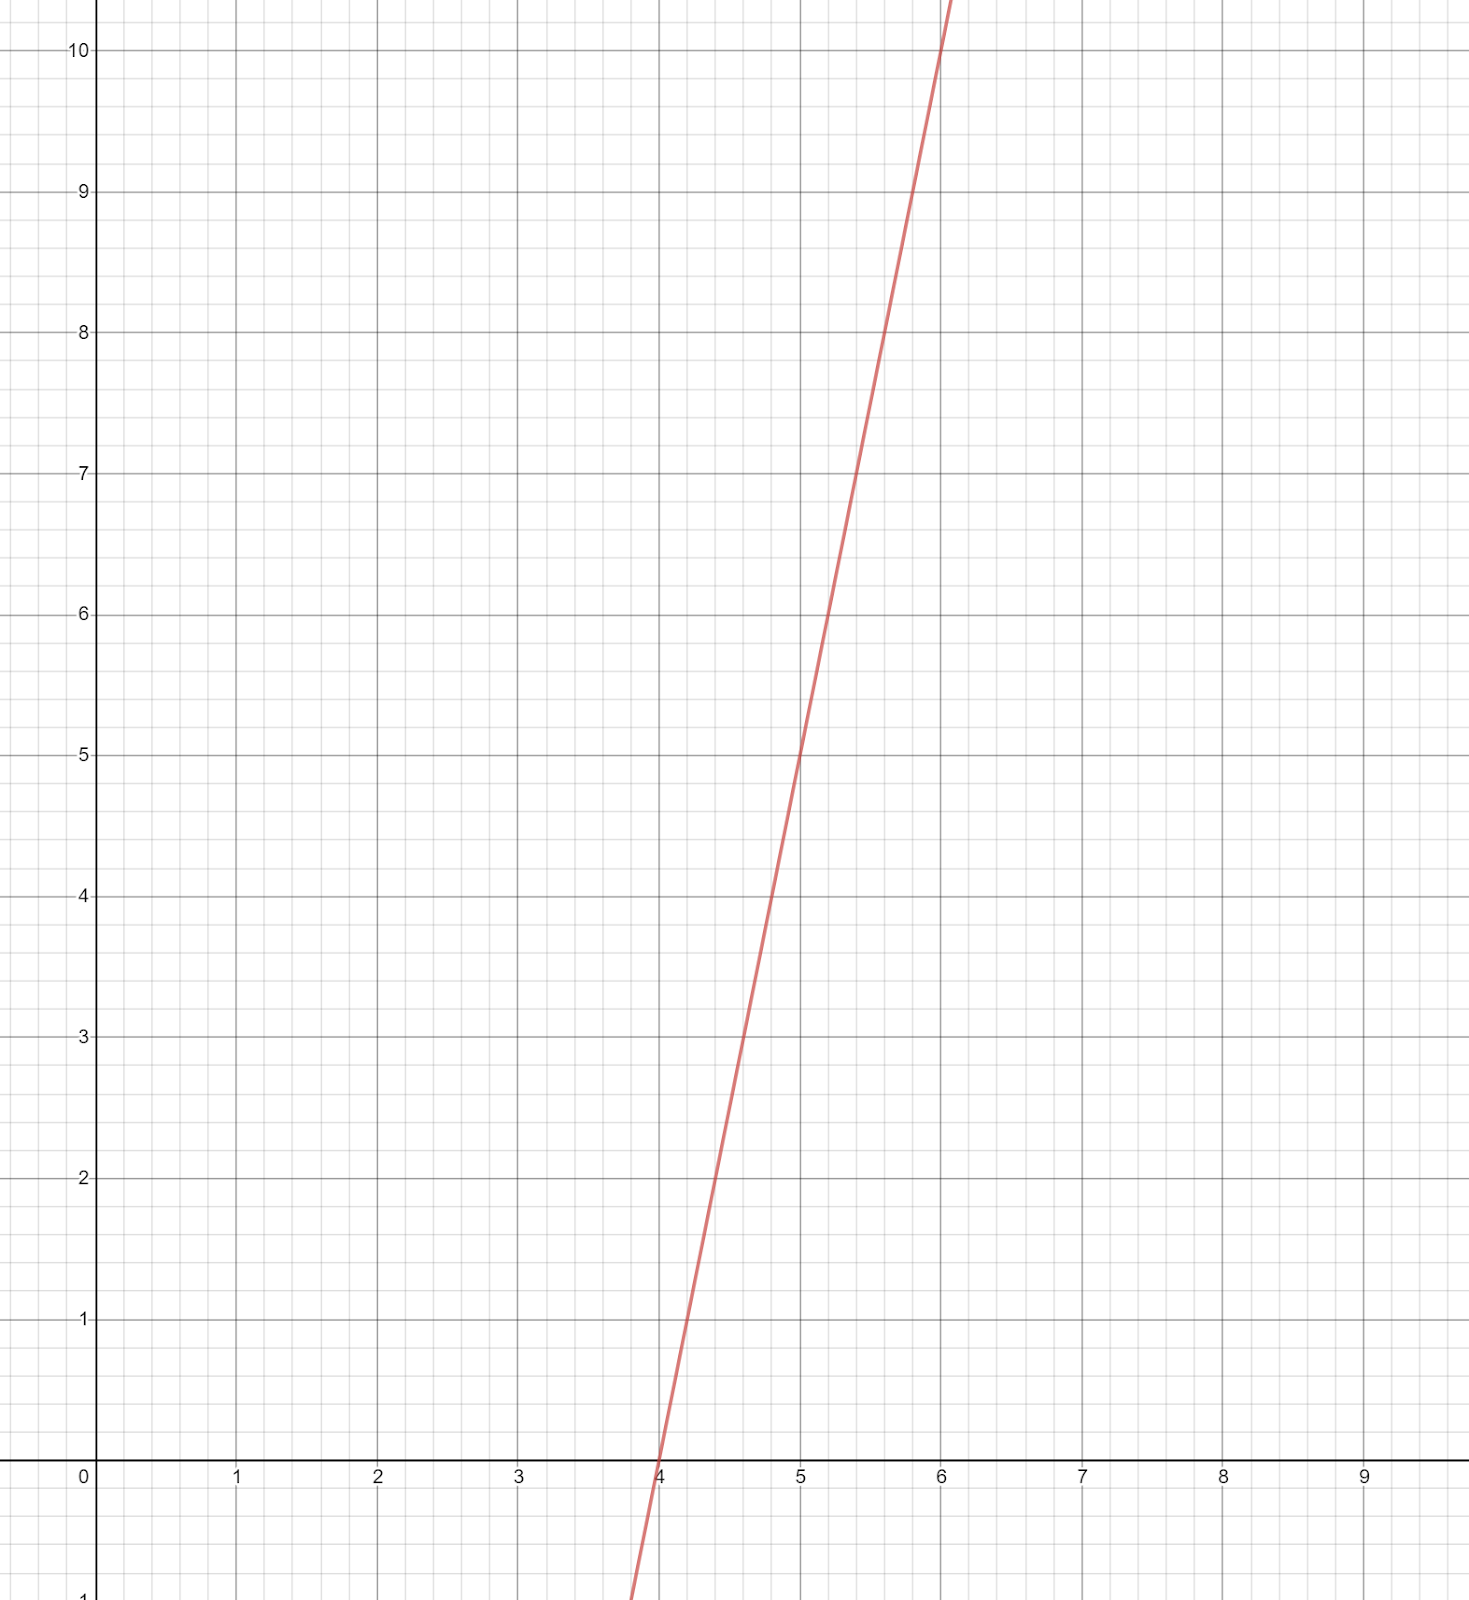
\includegraphics[scale=0.1]{arima1}
    \caption{Plotting the data }
\end{figure}
The image above shows an implementation of auto regression on FTSE 100 data from 2010 to 2020. Green dots represent the predicted values while the red dots represent the actual values.
\clearpage
\begin{figure}[h]
    \centering
    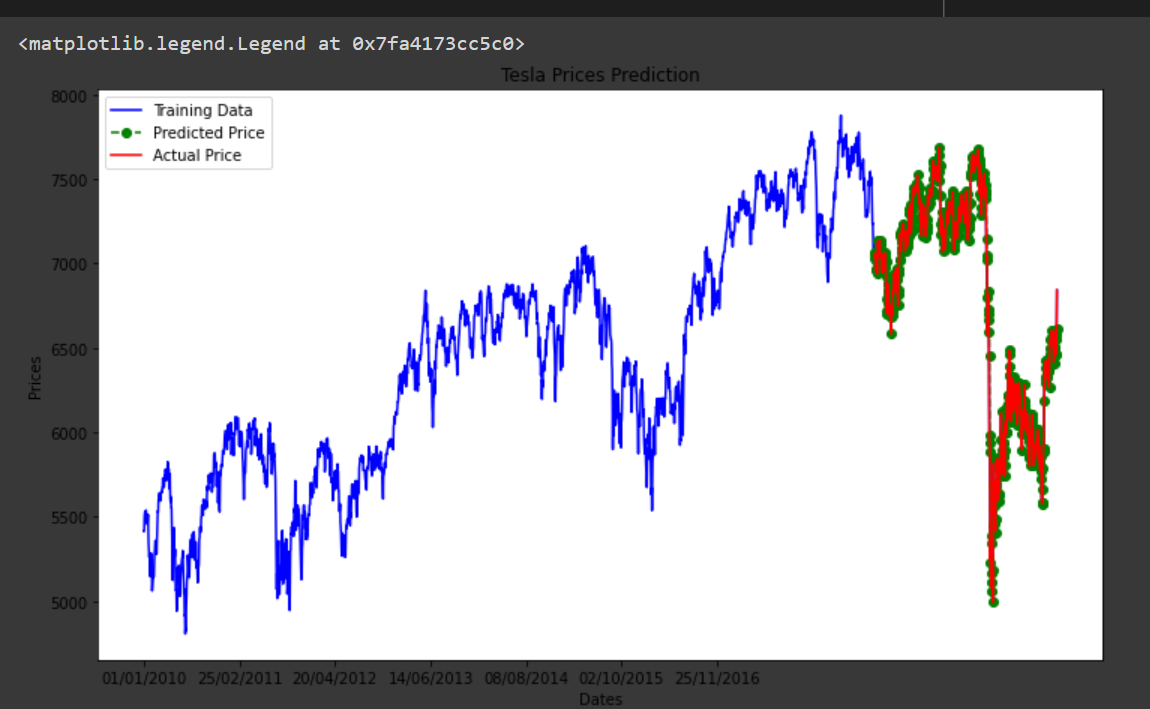
\includegraphics[scale=0.21]{arima2}
    \caption{Using ARIMA on test data }
\end{figure}
Figure 3 shows the accuracy of the model at a respectable 89.21\% when using MSE as the loss function.
\begin{figure}[h]
    \centering
    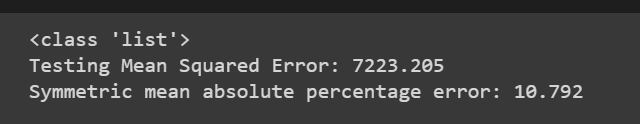
\includegraphics[scale=0.35]{arima3}
    \caption{MSE Loss using ARIMA }
\end{figure}

\subsection{Neural Networks}
The research done in the 1990s have helped set up the foundations for a mathematical model that is today known as machine learning. This mathematical process aims to replicate the brain through the use of several functions and calculus. This replication comes in the form of neurons in a neural network. In the following paragraphs I will proceed to explain a type of neural network known as a ‘Convoluted neural network’ before proceeding to describe an evolution, the ‘Recurrent neural network’.


\subsection{CNN}
The neural network is heavily dependent on the maths surrounding gradients, in particular differentiation. The main components of a neural network include: an activation function, layers, a loss function and an optimiser.
\\
Similar to the human brain, a neural network is made up of many neurons. These neurons are information processing units that are fundamental to the operation of a neural network. The structure of a neuron is shown in figure 2.2.3 and is represented by a subscript k.  A basic neural network consists of 3 main parts: a set of connecting links between neurons, an adder and an activation function.
\\
The set of links each have a weight assigned to them. They work by taking input signals, often as vectors, and then multiply these by the weights they are assigned. This process is shown in figure 2.2.3. After that each vector is added together before a fixed bias is applied. To simulate the process of a neuron turning on and off, an activation function is used. These are mathematical functions and are described in the following paragraphs.

\subsection{Activation Functions}
To summarise the behaviour of an activation function, it can be compared to a transistor; it only activates at a certain threshold.  These try to replicate how the neurons behave in our brain.
The most common activation functions are shown below along with their equation.

\begin{itemize}
    \item Binary step function
    \begin{itemize}
        \item \begin{align*}
            u(x) = 	1 \mbox{ if }  x \geq 0 \mbox{ or } 0 \mbox{ if } x <  0
        \end{align*}


     \begin{align*}
            Y = u(x-3)
        \end{align*}
        \begin{figure}[h!]
            \centering
            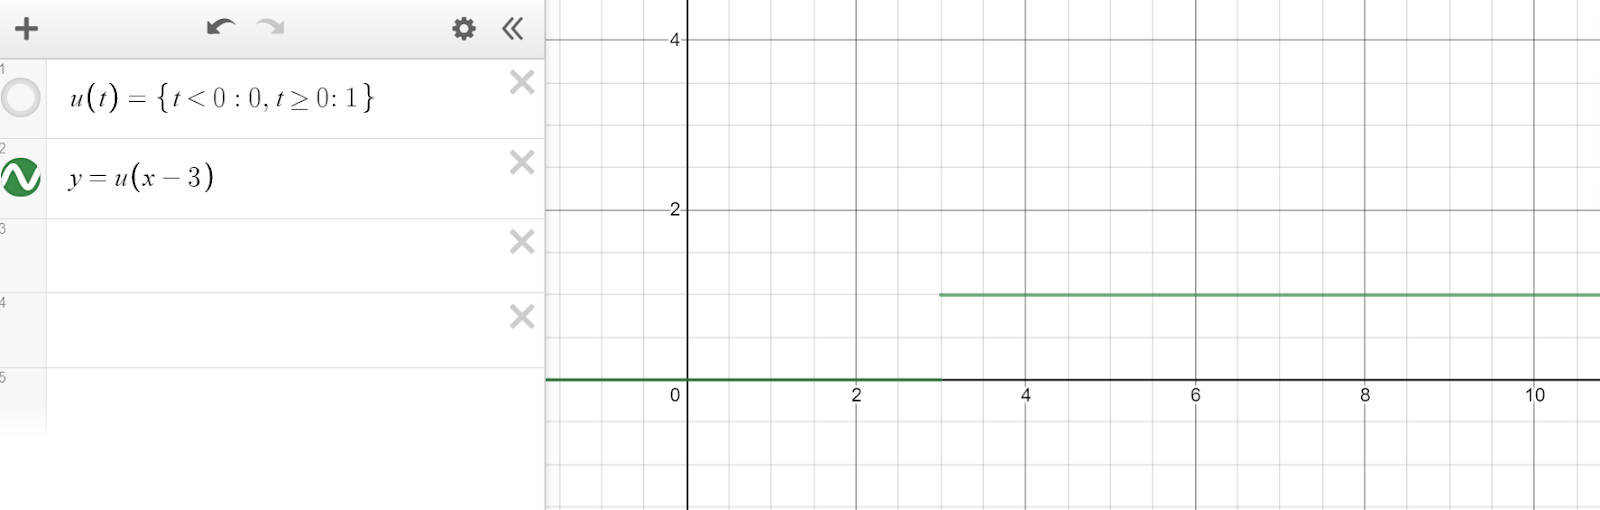
\includegraphics[scale=0.15]{binarystep}
            \caption{Binary step function}
        \end{figure}
    \end{itemize}


    \item Linear Function
        \begin{itemize}
            \item \begin{equation*}
            f(x) = mx
        \end{equation*}
        \end{itemize}


    \item Sigmoid
        \begin{itemize}
            \item
        %Values range from 0 to 1\\
        %\begin{align*}
            $$\sigma(x)  =\:\frac{1}{\:1+e^{-x}}$$
            $$\frac{d}{dx} =$$
            $$f  = 1 \quad f' = 0$$
            $$g  = 1 + e^{-x} \quad g' = -e^{-x}$$
            Using the quotient rule:
            $$= \frac{e^{-x}}{{(1+e^{-x})}^2}$$
        %\end{align*}
            This can also be written as:
            $$\sigma'(x) = \sigma(x)(1-\sigma(x))$$

        \end{itemize}


    \item Tanh
        \begin{itemize}
        \item $tanh(x) = 2\sigma(2x)-1$
        \itme Values range from -1 to 1
        \end{itemize}
        \begin{figure}[h!]
            \centering
            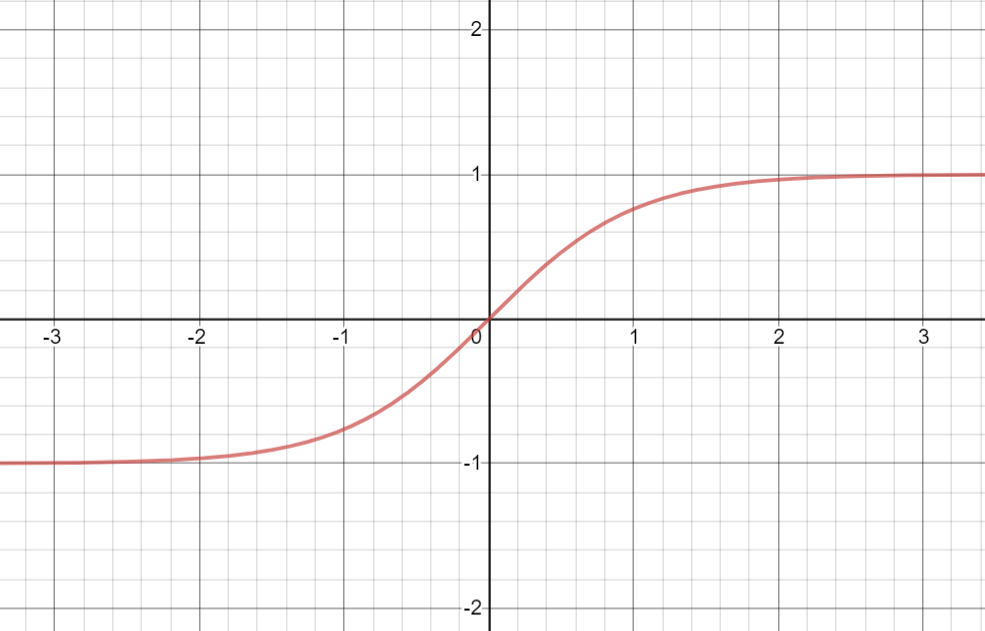
\includegraphics[scale=0.15]{tanh}
            \caption{Tanh function}
        \end{figure}


    \item ReLU(Rectified Linear Unit)
        \begin{itemize}
            \item Neurons will only deactivate if the output of the linear transformations less that 0\\
            Also a leaky version of ReLU present
        \end{itemize}
        \begin{figure}[h]
            \centering
            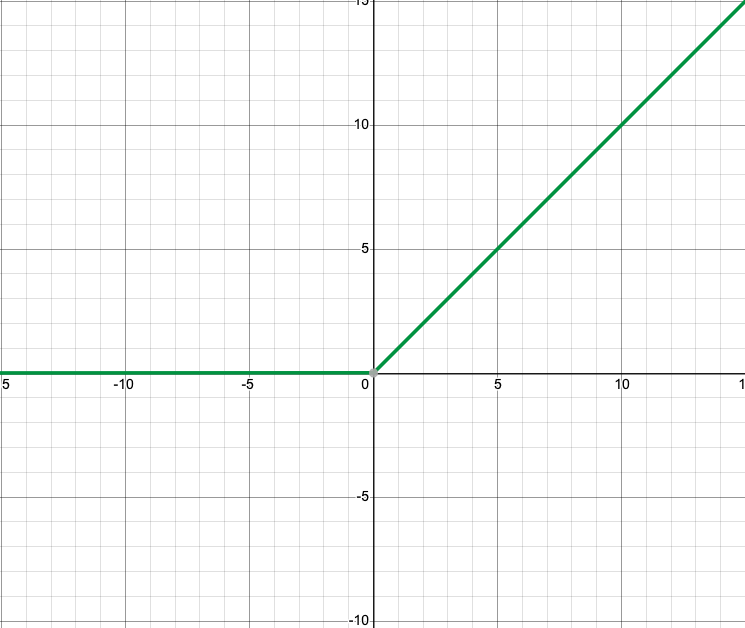
\includegraphics[scale=0.15]{relu}
            \caption{ReLU function}
        \end{figure}

    \item Softmax
        \begin{itemize}
            \item Returns the probability for a data point belonging to each individual class
            $$\sigma(\hat{z})_i = \frac{e^{zi}}{\sum_{j=1}^{k}e^{z_j}}$$
            Below is a description of the softmax function: (Versloot, 2020)\\

This can be described as the following: for each value in our input vector, the Softmax value is the exponent of the individual input divided by a sum of the exponents of all the inputs.
\\
This ensures that multiple things happen:
\\
Negative inputs will be converted into nonnegative values, thanks to the exponential function.\\
Each input will be in the interval (0,1)
As the denominator in each Softmax computation is the same, the values become proportional to each other, which makes sure that together they sum to 1.\\
\\
These properties allow us to interpret them as probabilities.
\\
To make sure these values are actually valid probabilities, it can be checked against Kolomogorov’s probability axioms.
\begin{itemize}
    \item Each probability must be a nonzero real number. This is true for our outcomes: each is real-valued, and nonzero.
    \item The sum of probabilities must be 1. This is also true for our outcomes: the sum of cutoff values is$\approx$ 1, due to the nature of real-valued numbers. The true sum is 1.
\end{itemize}
Here is an example of the function
\begin{figure}[h!]
            \centering
            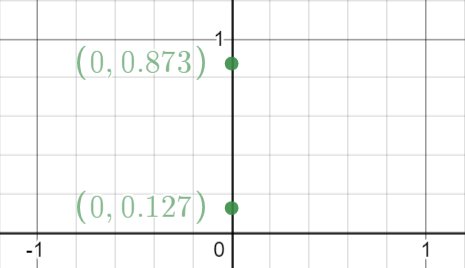
\includegraphics[scale=0.25]{softmax}
            \caption{Where a = 6.638 and b = 4.71}
        \end{figure}
        \end{itemize}
        In the equation above, $\hat{z}$ is the input vector to the softmax function, made up of ($z_0, ... z_k$)\\
        $z_i$ are All the $Z_i$ values are the elements of the input vector to the softmax function, and they can take any real value, positive, zero or negative. For example a neural network could have output a vector such as (-0.62, 8.12, 2.53), which is not a valid probability distribution, hence why the softmax would be necessary.\\
        $e^{z_ii}$ is the  standard exponential function is applied to each element of the input vector. This gives a positive value above 0, which will be very small if the input was negative, and very large if the input was large. However, it is still not fixed in the range (0, 1) which is what is required of a probability.\\
$\sum_{j=1}^{k}{e^{z_j}}$ is the term on the bottom of the formula is the normalization term. It ensures that all the output values of the function will sum to 1 and each be in the range (0, 1), thus constituting a valid probability distribution.\\
        $k$ is the number of classes in the multi-class classifier.
\end{itemize}
\item ELU(Exponential linear unit)\\
The exponential linear unit was designed to fix some of the problems with ReLUs. This function has a parameter that is picked; a common value is between 0.1 and 0.3.
\begin{equation*}
            ELU(x) = 	x \mbox{ if }  x > 0 \mbox{ or } \alpha(e^{x}-1)  \mbox{ if } x <  0
        \end{equation*}
This  equation tells us that if the input, x, is greater than 0 then the output is the same as a RELU, y=x. If the input drops below 0, the value becomes slightly smaller than 0. This value will be modelled using (ex-1)where we choose a value for . The exponential operation makes this function more computationally expensive than a vanilla ReLU. The exponential function helps fix the vanishing gradient problem often associated with ReLUs. An advantage is that the ELU produces negative values which allows them to push mean unit activation close to zero, a bit like batch normalisation but with lower computational complexity. Mean shifts towards zero help speed up learning.
\begin{figure}[h!]
            \centering
            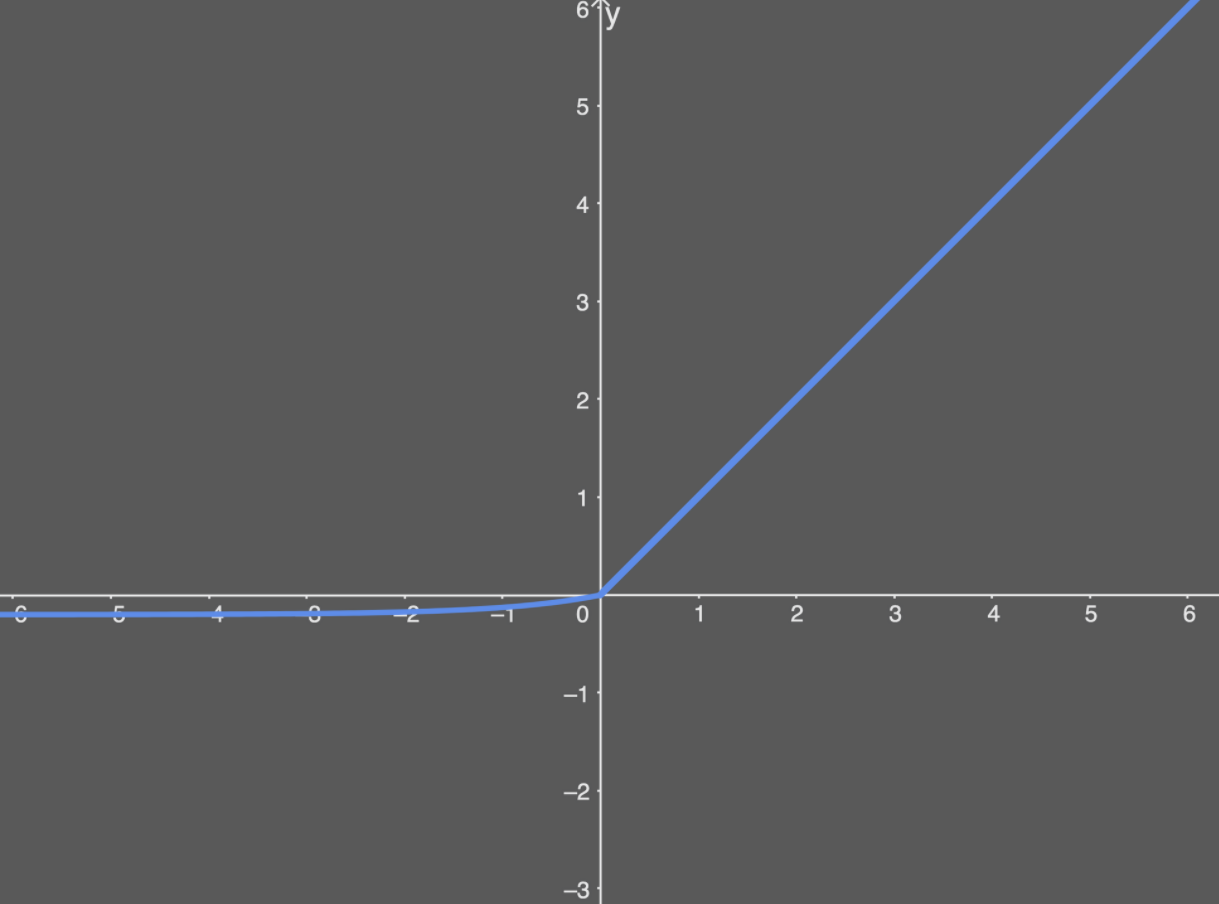
\includegraphics[scale=0.15]{elu1}
            \caption{ELU function}
        \end{figure}
The derivative can be written as\\
\begin{equation*}
            ELU'(x) = 	1 \mbox{ if }  x > 0 \mbox{ or } \alpha(e^{x})  \mbox{ if } x <  0
       \end{equation*}
The exponential function helps make this function differentiable at all points.  Below is the graph for the derivative:
\begin{figure}[h!]
            \centering
            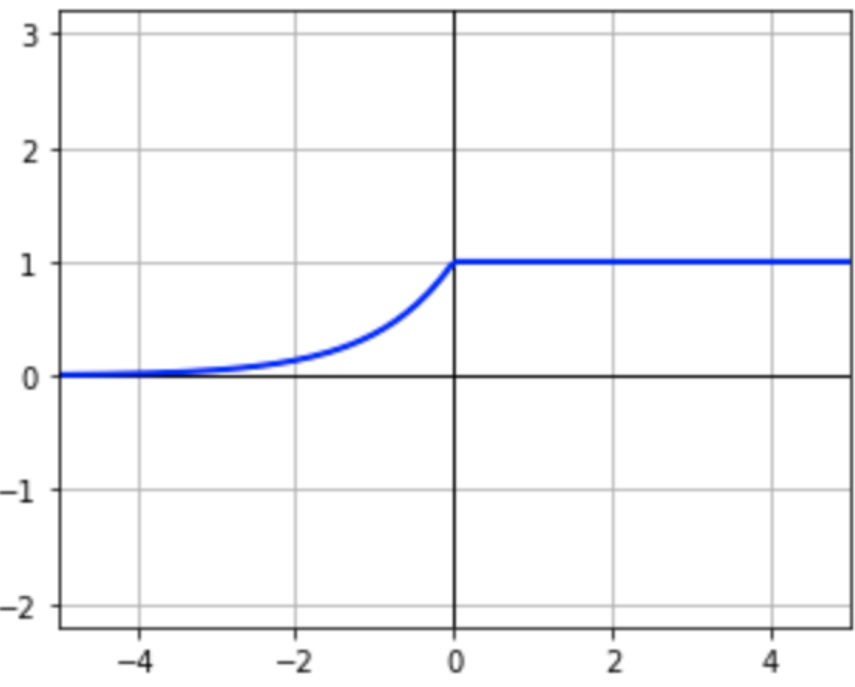
\includegraphics[scale=0.15]{eluderiv}
            \caption{ELU derivative function}
        \end{figure}

\end{itemize}

\subsection{Layers}

As shown in the figure below, in between the input and output layers there are hidden layers.  These layers contain many neurons. The equation that is used to model these neurons is shown in the second image, I have used the sigmoid function as an example of the calculation that may happen at a neuron. The summation of the weights multiplied by the input activity. A bias is then applied before the activation function, a sigmoid in my example, is applied to the result to determine whether the neuron should turn on or not.
\begin{figure*}[h!]
            \centering
            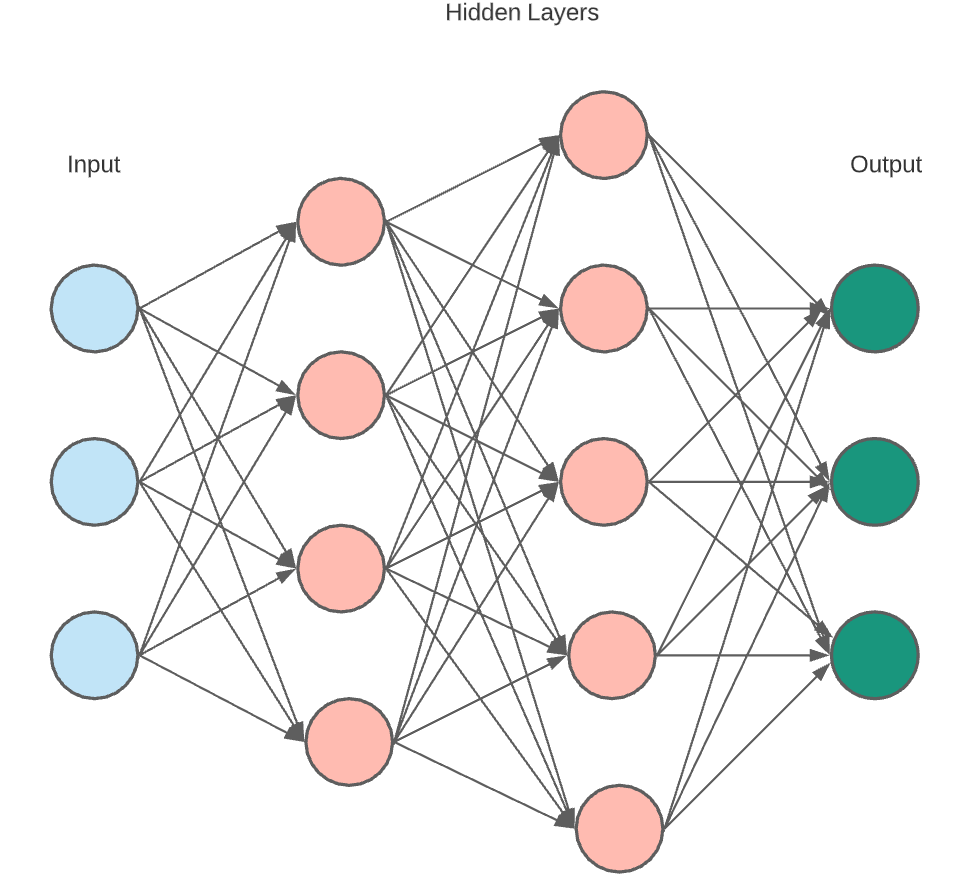
\includegraphics[scale=0.15]{layers1}
            \caption{Layers shown in a neural network}
        \end{figure*}
\begin{figure}[h!]
            \centering
            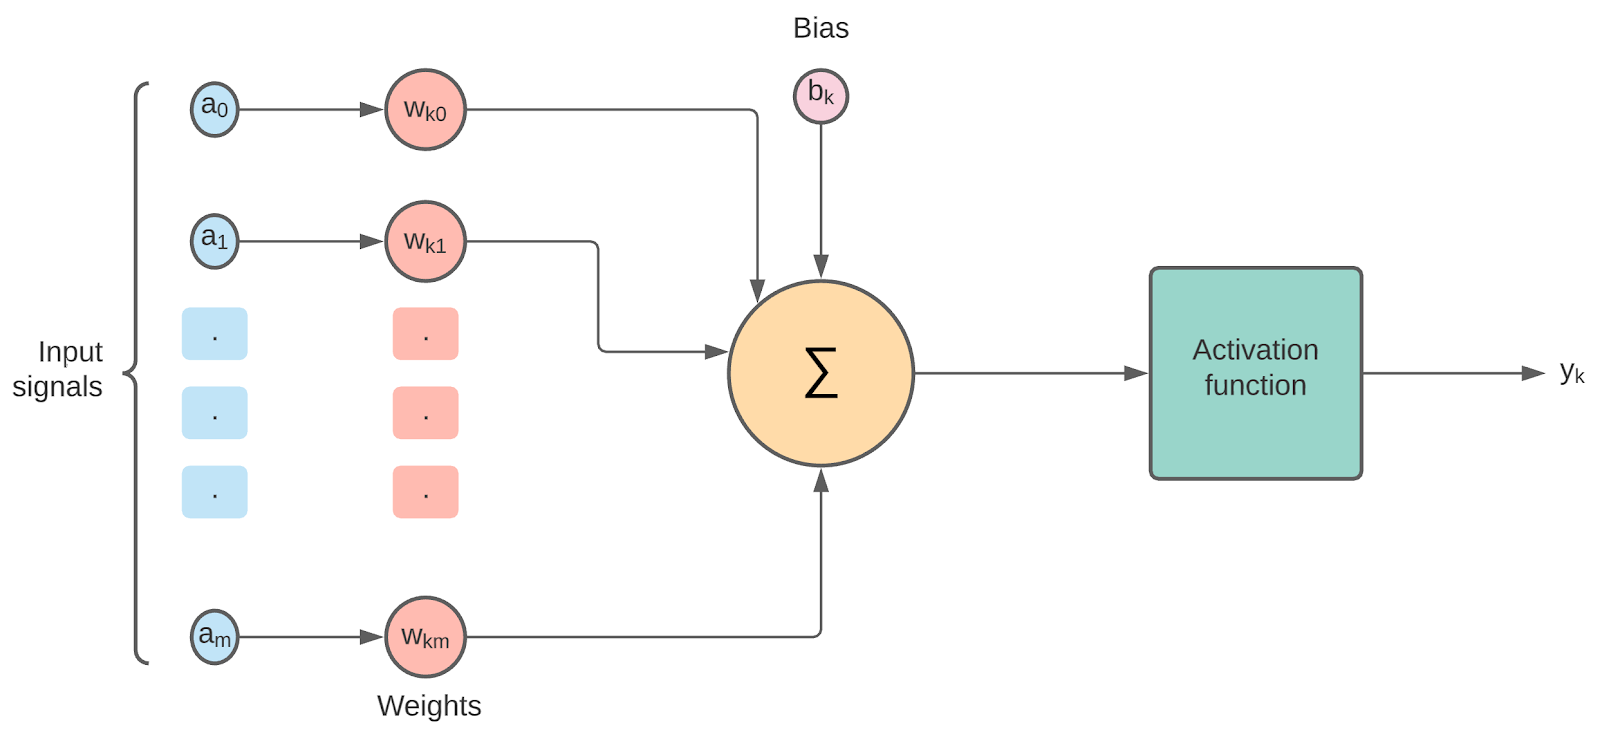
\includegraphics[scale=0.15]{layers2}
            \caption{Neuron represented mathematically}
        \end{figure}

\subsection{Neurons and Equations}
The neurons can be modelled using the equations given below in the equation $$a = \sigma(w \times a + b)$$
Here $a$ is the activity, the activity of the neuron, $\sigma$ is the activation function, $w$ is the weight and $b$ is the bias.
The equation shows that the activity is modelled by multiplying the previous activity by a weight that is changed during the whole learning process, before a constant bias is applied. The equation below shows a more general equation where the letter L represents a neuron in current time and so L-1 is the activity of the previous neuron.
$$a^{L} = \sigma(w^{L}\times a^{L-1} + b^{L})$$
Another way to write this is:\\
$$\sigma((\sum_{j=0}^{n}w_j\cdot a_j)+b)$$

\subsection{Loss Functions}

A loss function is what ultimately gives the neural network its intelligence. At its core it’s a method evaluating how well the algorithm models the data. If the predictions are off by a high margin then a high loss will be calculated. If the margin of error is lower, a lower number will be calculated showing that your predictions are quite close. This loss is also commonly referred to as the accuracy. The goal is to get your loss as low as possible or can be referred to as achieving a high accuracy.  There are many functions that can be used to determine the loss but the most common are root mean squared error, absolute error loss and binary cross entropy loss. Lots of neural networks have custom loss functions that are dependent on the purpose they are serving. A very strict loss function that amplifies the loss is more typical in places where the loss must be kept at a minimum such as stock prediction.

\subsection{Feed Forward and Back propagation}
For the neural network to truly learn, it must go through a process called back propagation. This is an algorithm that is used in supervised learning and uses a concept called gradient descent.
One way to think about a loss function is to imagine it being a black box that works out an equation, say y =  to get you from the domain to the range. Now this equation can be plotted, figure 2 and we can see that there are a few things to observe about this graph. Calculus tells us that the turning points happen when the gradient of a curve, that can be worked out using differentiation, is 0. The second step is to work out the second derivative and that will  tell us whether the point is a maxima or minima. Where $\frac{d^{2}y}{dx^{2}} > 0$, the point can be described as a minimum and when $\frac{d^{2}y}{dx^{2}} < 0$, the point can be described as a maximum. The minimum point that occurs when $\frac{dy}{dx}$ (the gradient)is 0, on the graph below it happens at the point (3,0).

\begin{figure}[h!]
            \centering
            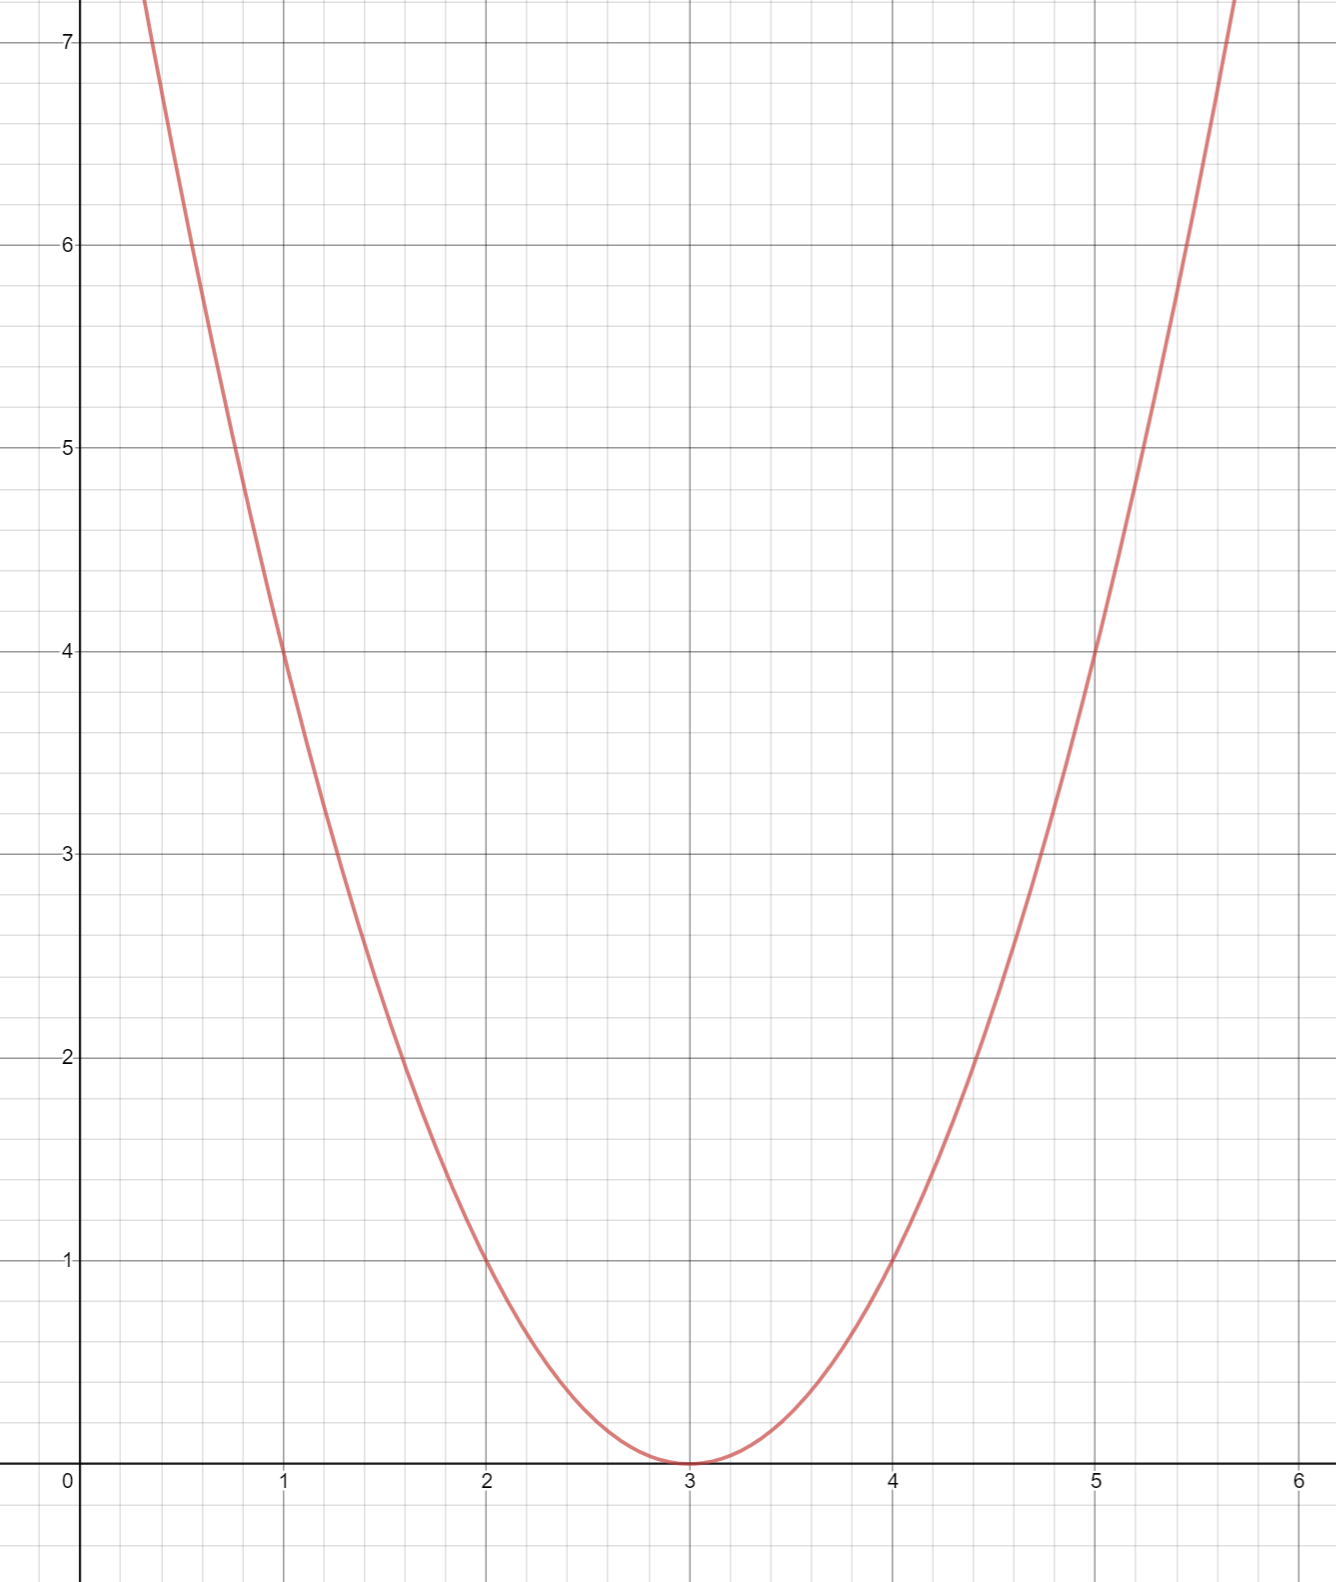
\includegraphics[scale=0.15]{ff1}
            \caption{}
        \end{figure}
Consider $w$ to be one of the weights discussed in the previous section.\\
If $w<3$, we have a positive loss function, but the derivative is negative, meaning that an increase of weight will decrease the loss function.\\
At $w=3$, the loss is 0 and the derivative is 0, we reached a perfect model, nothing is needed.\\
If $w>3$, the loss becomes positive again, but the derivative is as well positive, meaning that any more increase in the weight, will increase the losses even more.\\
To try and decrease this loss, at $w<3$ you should increase the weight and at $w>3$ you should decrease the weight.\\
\\
The equation for working out the new weight is shown below where $w_n$ is the weight, $C$ is the cost function and $\alpha$ is the learning rate(which is a constant). \\

$$new\hspace{3}w_n = (old\hspace{3} w_n) - \alpha \cdot \frac{\partial C}{\partial w_n}$$
%error above, not too sure why

\subsection{Backpropagation}
The goal of backpropagation is to minimise the error function by changing the weights of the individual neurons. The formulation of the complete backpropagation algorithm can be proven by induction to show that it works with differentiable activation functions at its nodes.
\\
For this proof, the assumption has been made that the neural network is one with a single input and single output. To simplify the proof, instead of carrying a bias term, let us assume that each layer $V^{(t)}$ contains a single neuron $v_o^{(t)}$ that always outputs a constant 1 thus the output of a neuron is given by $$\sigma(\sumw_{i,j}v_j^{t-1})$$ We next wish to compute the derivative $\nabla f_w$. Now suppose neuron $v_i^{t}$ computes:
$$v_i^t(x) = \sigma(u_i^t(x))$$
Then using the chain rule we can obtain that\\
$$\frac{\partial f}{\partial w_{i,j}} = \frac{\partial f}{\partial u_i^t}\cdot \frac{\partial u_i^t}{\partial f} = \frac{\partial f}{\partial u_i^t}v_i^{(t-1)}(x)$$\\

Thus to compute the partial derivative of a single weight, it is enough to compute $\frac{\partial f}{\partial u_i^t}$.
We can now focus on computing $\frac{f}{\partial u_i^t}$. Now suppose f is a function of $u_1^t, \cdots, u_m^t$, which we are in turn function of some variable $z$ then we have by chain rule:
$$\frac{\partial f}{\partial z} = \sum_{i=1}^{m}\frac{f}{\partial u_i^t}\cdot \frac{\partial u_i^t}{\partial z}$$
Now if $z = u_n^{t-1}$ is the output of some neuron in a previous layer: The calculation of $\frac{u_i^t}{\partial u_n^{t-1}}$ is easy for our choice of activation function
$$u_i^t = \sum w_{i,j}\sigma(u_j^{t-1}) \rightarrow \frac{u_i^t}{u_n^{t-1}} = w_{i,n}\sigma'(u_n^(t-1))$$
Using this equation for $f= u_i^t$ we can recursively calculate all the partial derivatives. This inductive approach can be used to calculate all the dervatives, giving us the backpropagation algorithm. In reality the algorithm calculates the derivatives through dynamic programming therefore reducing the complexity.\\
To summarise the process consider an input-output pair, (x,y). Use the current set of weights at
t=0 in the network to generate the output vector $g(x)$, whose individual values comprise of the $a_N$
values for each neuron in the output layer. Next compute the derivatives for each neuron in the
output layer and use those values to update the weights ,$w$, on the incoming edges on the graph
for those neurons using the update rule. Next, for the neurons in the last hidden layer, the layer
before the output layer, compute the derivatives then use them to update the incoming edges for
those neurons. Repeat this process for each neuron in the network. Eventually you will reach the
input layer where there are no incoming edges and hence no weights to update.
This process should be done for each input-output pair in the training data.\\
In testing a standard Seq-Seq CNN displayed an accuracy of 90.7\%.(Zolkepli and Divino, n.d.).
This is slightly higher than the ARIMA model but is still not satisfactory for use in the stock
market.
\subsection{RNN}
The traditional CNN started to become of great interest in the 2000s and started to evolve to fit
many purposes. One such evolution is into the recurrent neural network.\\
Recurrent neural networks were created because there were a few issues with the standard feed
forward CNN. The issues came about as the input started to change from just being a few
numbers to images represented as a matrix. The main issues were that it couldn’t handle
sequential data, only considered the current input and that it couldn't memorise previous inputs
An RNN works on the principle of saving the output of a particular layer and then feeding this
back to the input in order to predict the output of the layer. This gives them the ability to
remember their last input.\\
\begin{figure}[h!]
    \centering
    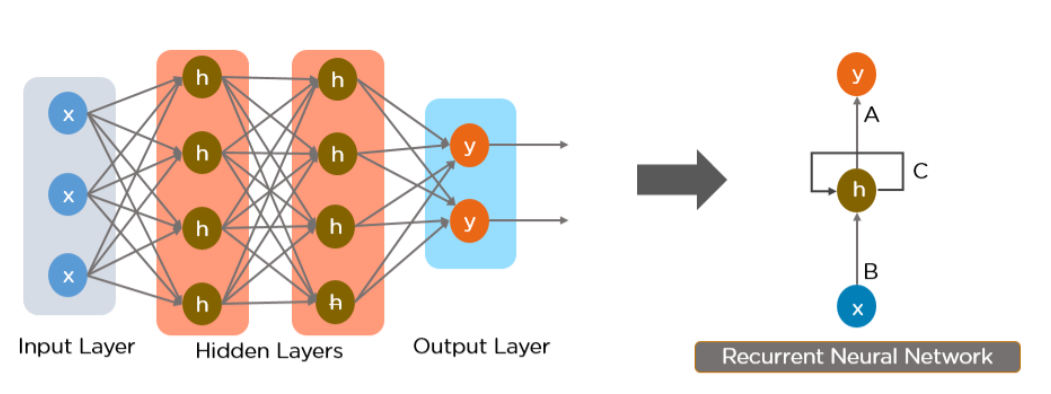
\includegraphics[scale=0.15]{rnn1}
    \caption{RNN visualised }
\end{figure}
\begin{figure}[h]
    \centering
    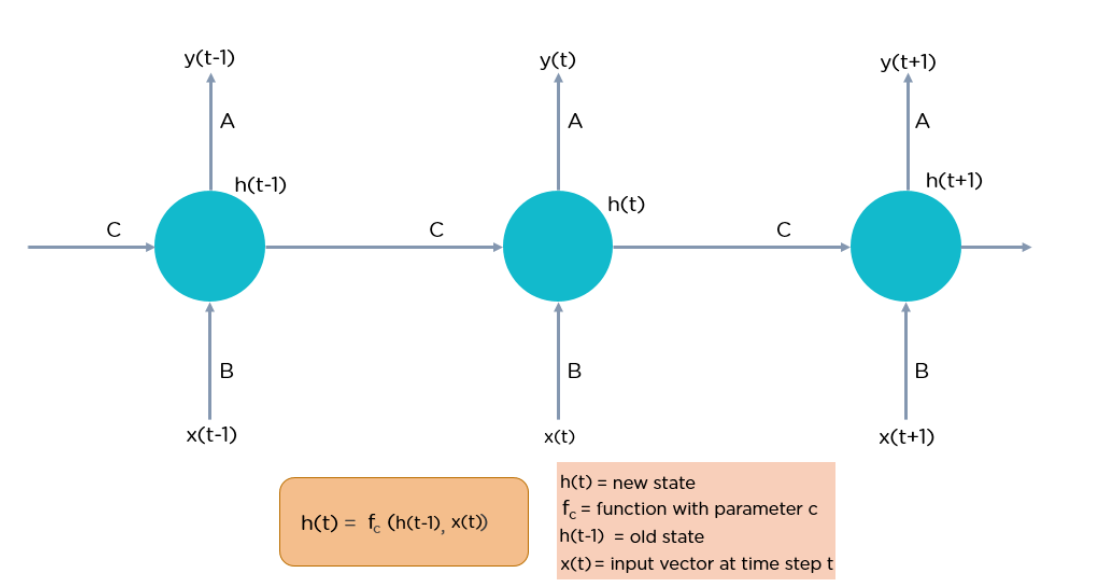
\includegraphics[scale=0.15]{rnn2}
    \caption{RNN broken down into individual components }
\end{figure}
\begin{figure}[h]
    \centering
    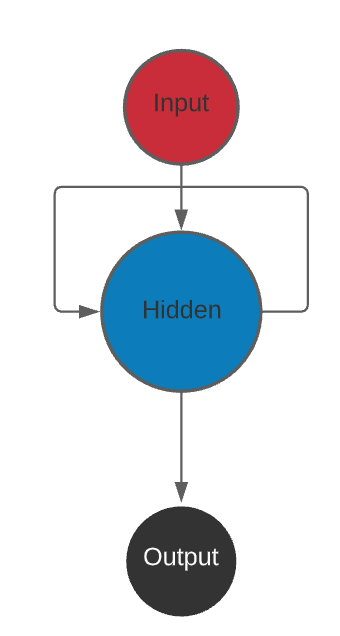
\includegraphics[scale=0.15]{rnn3}
    \caption{}
\end{figure}
\subsubsection{Problems with RNN}
The RNN has two big problems: a vanishing gradient problem and an exploding gradient
problem.\\
As previously mentioned, the gradient descent algorithm finds the minimum of a function to
find the optimal weights.\\
In RNNs, information first travels through time which means that information from previous
time points is used as the input for the next time points. Secondly the cost/error function is
calculated at each time point.\\
Essentially, every single neuron that participated in the calculation of the output, associated with
this cost function, should have its weight updated in order to minimize that error. And the thing
with RNNs is that it’s not just the neurons directly below this output layer that contributed but
all of the neurons far back in time. So, you have to propagate all the way back through time to
these neurons.\\
The problem relates to updating wrec (weight recurring) – the weight that is used to connect the
hidden layers to themselves in the unrolled temporal loop.\
For instance, to get from xt-3 to xt-2 we multiply xt-3 by wrec. Then, to get from xt-2 to xt-1 we
again multiply xt-2 by wrec. So, we multiply with the same exact weight multiple times, and this
is where the problem arises: when you multiply something by a small number, your value
decreases very quickly.\\
As we know, weights are assigned at the start of the neural network with the random values,
which are close to zero, and from there the network trains them up. But, when you start with
wrec close to zero and multiply xt, xt-1, xt-2, xt-3, … by this value, your gradient becomes less
and less with each multiplication.\\
(Biswal, 2021)

\subsection{LSTM}
All RNNs have feedback loops to help them maintain the information in the memory while
training but to resolve the problems mentioned above, the LSTM was created.
Long-short term memory networks are a type of RNN that introduces the use of gates such as
input and forget gates which allow for better control ive the gradient flow hence allowing a
better preservation of long-range dependencies. These gates use functions that we have
mentioned before such as the tanh function, and the sigmoid function.
\begin{figure}[h!]
    \centering
    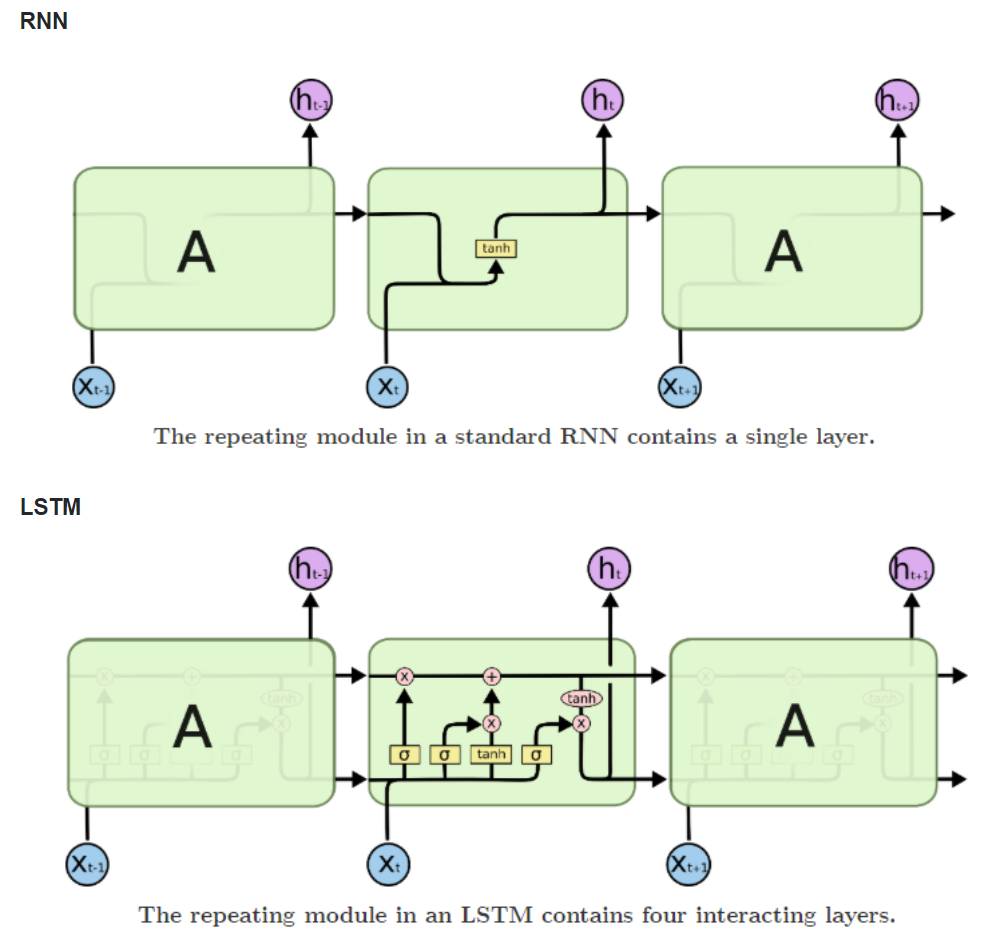
\includegraphics[scale=0.15]{lstm1}
    \caption{}
\end{figure}
(Olah,2015)
The LSTM has a block called the cell state, the middle block in the diagram above. The network
has the ability to remove or add information to the cell state so that it can be accessed at a later
time. This cell state is protected by the mathematical functions so that it doesn’t get cluttered
with useless information
\subsubsection{Problems with LSTM}
As you can see from the image above, there is a sequential path from the oldest past cells to the
current ones. This sequential path is now more complex with the addition of forget gates. This
makes them very resource intensive and so requires an immense amount of memory. This makes
them very inefficient and so unsuitable for small devices such as home devices like Amazon
Echo or Apple home pods.\\
LSTMs also get affected by different random weight initialisations and hence act just like a nomla
feed forward neural network with extra steps making them nearly useless. They much prefer
small weight initialisations.\\
Along with these problems, LSTMs are prone to overfitting and are difficult to apply dropout
algorithms to resolve this issue. To add to this list is the fact that LSTMs struggle to retain
information when handling larger datasets. They can handle sequences of 100s but not 1000s or above. This makes them unsuitable for tasks like stock prediction or neural language processing.

\subsection{Transformers}
The Transformer is an evolution of the RNN and its main purpose was to solve the problem of
parallelisation. It only performs a small, constant number of steps. In each step it applies a
self-attention mechanism that helps it retain information for longer making it more suitable for
larger datasets. This model is typically used for neural language processing where keeping a
track of all the words used helps the machine to gain understanding about the context. A
common neural network would typically contain an encoder that would read the input sentence
and would generate a representation of it. A decoder would then generate the output sentence
while looking back to the representation the encoder created. The Transformer takes a different
approach; it starts by generating initial representations/embeddings for each word. A self
attention mechanism is then applied to the representation which generates a new representation
for the word by comparing it to previous words. This step of making a new representation is
repeated multiple times in parallel for all the words in the input sentence.\\
This parallelisation increases its computational performance and produces a high accuracy.
\begin{figure}[h!]
    \centering
    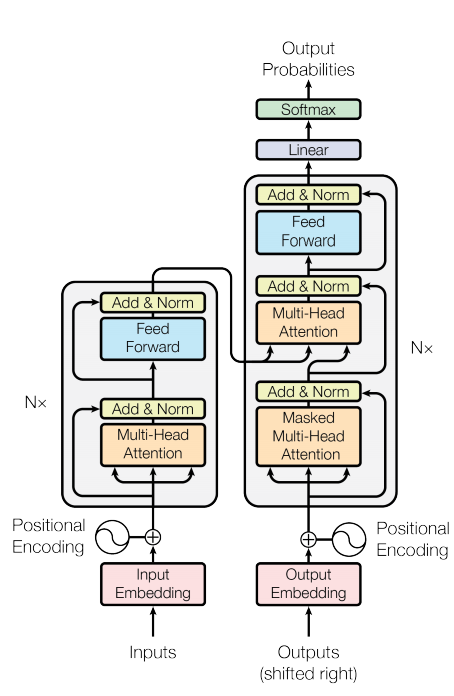
\includegraphics[scale=0.15]{transformer1}
    \caption{transformer model}
\end{figure}
(Vaswani et al., 2017)

\subsection{Attention}
(Lambda, 2019)
A critical and apparent disadvantage of this fixed-length context vector design is the incapability
of the system to remember longer sequences. Often it has forgotten the earlier parts of the
sequence once it has processed the entire sequence. The attention mechanism was born to resolve
this problem.\\
A neural network is considered to be an effort to mimic the brain in a simplified manner. The
attention mechanism can be described as an attempt to mimic the action of selectively
concentrating on a few relevant things instead of everything. There are two types of attention:
general attention and self-attention. General attention is between the input and output elements
and self-attention is within the input elements\\
The central idea behind attention is not to throw away any intermediate encoder states in LSTMs
and Transformers. Instead these states are used to construct the context vectors required by the
decoder to generate the output sequence.\\
A look into how self attention is calculated using vectors.\\
The first step in calculating self-attention is to create 3 vectors from each of the encoder’s input
vector, a query \boldsymbol{q}, a key \boldsymbol{k} and a value \boldsymbol{v}.\\
The second step is to calculate a score. The score determines how much focus to place on other
parts of the input as the input is encoded at a certain position.\\
The score is calculated by taking the dot product of the query vector with the key vector of the
respective value we are scoring. So if we are processing the self attention for the value in position
1 then the first score would be the dot product of $q_1$ and $k_1$. The second score would be the dot
product of $q_1$ and $k_2$.\\
The third step is to divide the scores by the square root of the dimension of the key vectors used.
This leads to having a more stable gradient.\\
This value will then be passed through the softmax function. This helps normalise the scores so
that they are all positive and add up to 1.\\
The fifth step is to multiply each value vector by the softmax score (in preparation to sum them
up). The intuition here is to keep intact the values of the word(s) we want to focus on, and
drown-out outliers (by multiplying them by tiny numbers like 0.001, for example).
The sixth step is to sum up the weighted value vectors. This produces the output of the
self-attention layer at this position for the first value.
\clearpage
\subsection{Temporal Fusion Transformers}
(Lim, 2020)
Attention is very useful for natural language processing but when handling time series data,
modifications have to be made. The temporal fusion transformer is the evolution made for this
type of data.
\begin{figure}[h!]
    \centering
    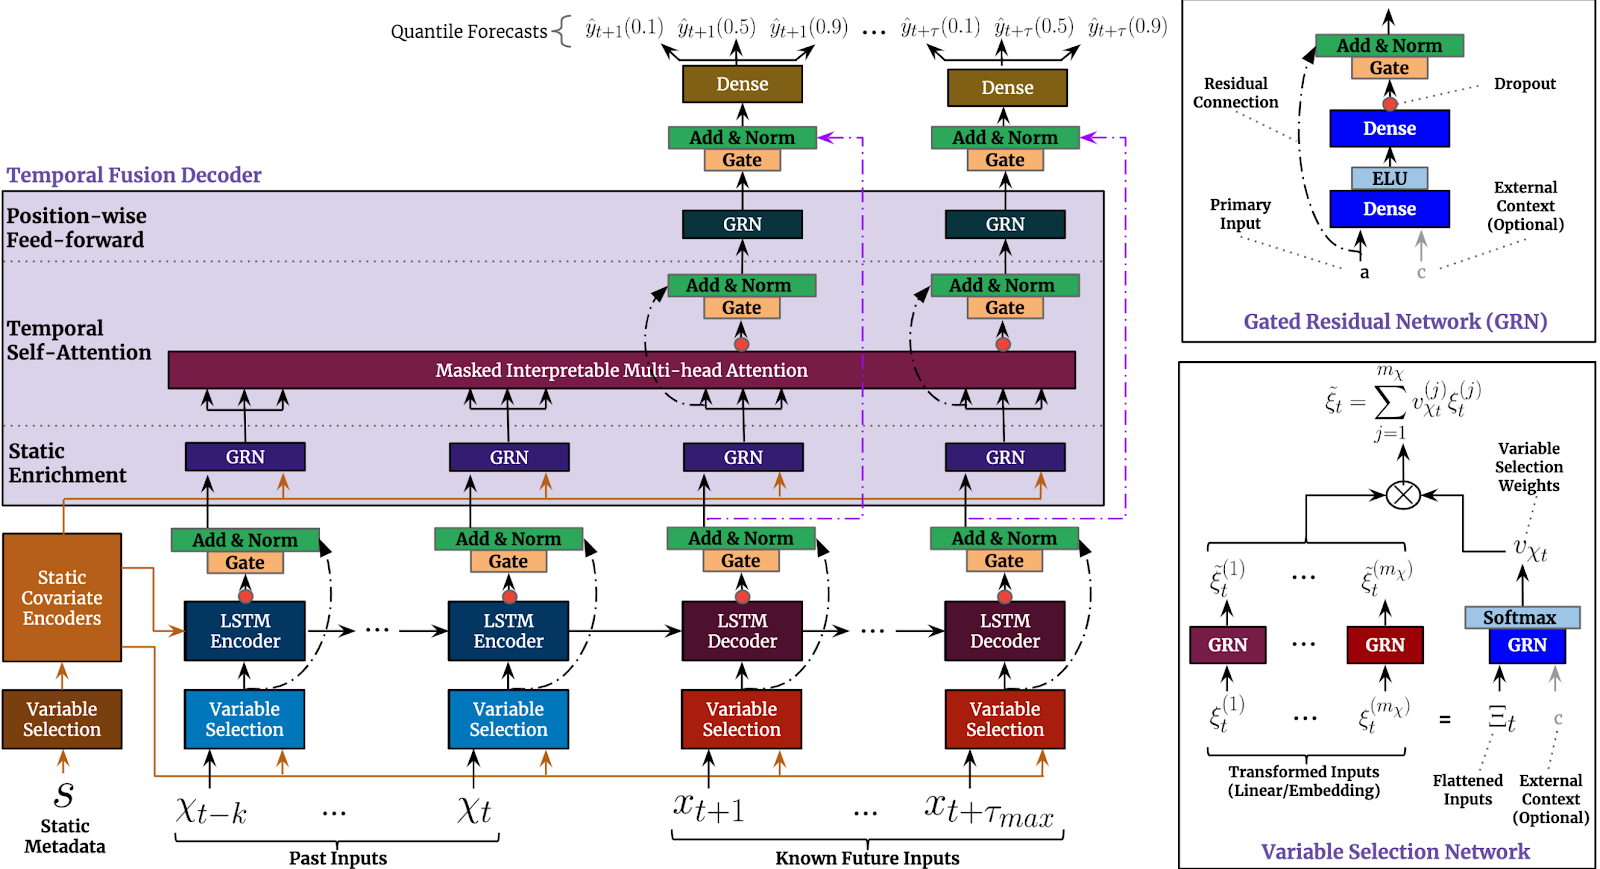
\includegraphics[scale=0.2]{tft}
    \caption{Temporal Fusion Transformer broken down into its components}
\end{figure}
The TFT has 5 main parts that get you from a dataset to a prediction. These allow the TFT to
efficiently predict future data points with a high performance.
\begin{enumerate}
\item Variable selection networks are used to select relevant input variables at each time step.
\item The gating mechanism to skip over any unused blocks and components of the architecture to allow for a dynamic model that adjusts itself to account for the dataset hence making it more time and memory efficient. This helps accommodate for larger datasets as well making the model more versatile.
\item The static covariate encoders are used to integrate start features into the network by encoding context vectors to condition temporal dynamics.
\item Temporal processing is used to learn both short and long term relationships between past and current inputs. Here a sequence to sequence layer with a multi-head attention block.
\item Prediction intervals via the forecasts to calculate the range of likely values at each step.
\end{enumerate}

\subsection{Tensors}
An $n$th-rank tensor in $m$ dimensional space is a mathematical object that has $n$ indicies and $m^n$ components that obeys certain transformation rules

\subsubsection{Tensor Product}
For any two vector spaces $\vec{U}$,$\vec{V}$ over the same field $F$, we can construct a tensor product $\vec{U}\otimes\vec{V}$ which is also an F-vector space.\\
Example:
$$\vec{v}=\begin{pmatrix}1\\ 2\\ 3\end{pmatrix}\quad \vec{w}=\begin{pmatrix}4\\ 5\end{pmatrix}$$
V is a vector in $\mathbb{R}^{2}$. W is a vector in $\mathbb{R}^{3}$.
$$\vec{v}\otimes\vec{v} \rightarrow \begin{pmatrix}1\cdot 4\\ 1\cdot \:5\\ 2\cdot \:4\\ 2\cdot \:5\\ 3\cdot \:4\\ 3\cdot \:5\end{pmatrix}=\begin{pmatrix}4\\ 5\\ 8\\ 10\\ 12\\ 15\end{pmatrix}$$

\subsection{Gated Linear Units(GLU)}
GLUs can be defined by the following equation:
$$h(x)=(x\cdot W +b)\otimes \sigma(X\cdot V+c)$$
Given a tensor, two independent convolutions are done and we get two outputs. We further do an additional sigmoid activation for one for the output, and find the tensor product of the two outputs.


\subsection{Gated Residual Network(GRN)}
\begin{figure}[h]
    \centering
    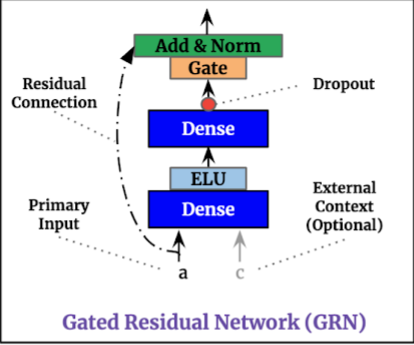
\includegraphics[scale=0.45]{grn}
    \caption{GRN visualised}
\end{figure}

The gated residual network, as shown in the image above,  consists of a dense block with an exponential linear unit as the activation function. This is then fed into another dense block before a GLU and normalised. There will be a connection between the input and output to allow for the attention mechanism to work. In my model, there will not be external context. The GRN can be modelled using the equations below:
$$GRN(\alpha) = LayerNorm(\alpha + GLU(\phi_1)) $$
$$\phi_1 = W_1, \phi_2+b_1$$
$$\phi_2 = ELU(W_2, \alpha + W_3) $$
$$\phi_1,\phi_2\in R $$

\subsection{Variable Selection Network}
\begin{figure}[h]
    \centering
    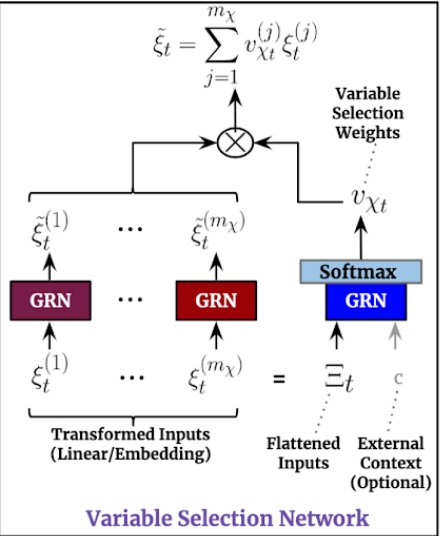
\includegraphics[scale=0.45]{vsn}}
    \caption{Variable Selection Network visualised}
\end{figure}

The purpose of the variable selection network is to evaluate the relevance of the variables than can be fed back into the model. This helps tell us what variables are the most significant as well as removing any unnecessary, noisy inputs that could negatively impact the performance of the model. This is useful when dealing with real time data as there might not be enough time to make sure all the data is correct or useful. As shown in the image above, there will be three GRNs with one of them having a softmax as the activation function. The tensor product will then be calculated.

\subsection{Multi-head attention}
The TFT model uses a self-attention mechanism to learn long term relationships between the data points across the different time steps. The concept of attention has already been explained and how that is calculated has also been discussed. To fit the TFT, a few modifications have been made. The general self-attention relies on the head value being the same but in our case this is different. This means the attention mechanism would have to only rely on the attention weights which is not enough. This problem has been solved by modifying the multi-head attention to share values in each head and using additive aggregation of all the heads.

$$MultiHead(\vec{Q},\vec{K},\vec{V}) = [\vec{H_1},...,\vec{H_h}]\cdot\vec{W_h} $$
$$ \vec{H_h}= Attention(\vec{Q}\vec{W_Q},\vec{K}\vec{W_K},\vec{V}\vec{W_V})$$
$$InterpretableMultiHead(\vec{Q},\vec{K},\vec{V})=\vec{\tilde{H}}\cdot\vec{W_H}$$
$$ \vec{\tilde{H}}=\tilde{A}(\vec{Q},\vec{K]})\cdot\vec{V}\vec{W_V}$$
$$=\frac{1}{H}\sum _{h=1}^{M_h}Attention(\vec{Q}\vec{W_Q},\vec{K}\vec{W_K},\vec{V}\vec{W_V})$$
The first equation shows what the equation would be when multiple heads are added. Q,K and V are the query vectors, key vectors and value vectors. Wv are the value weights shared across all the heads.
The interpretable multi-head function is our modified equation. The last equation shows us how we have employed additive aggregation.

\subsection{Quantile Forecasts}
The TFT can generate prediction intervals as well as point forecasts. This is done by predicting various percentiles (10\%, 50\%, 90\%) at each time step. The quantile forecast is calculated using the outputs of the temporal fusion decoder as is written as this:
$$\tilde{\xi} = GRN(\xi)$$
$$\phi(t,n)=LayerNorm(\tilde{\xi}+ GLU(\phi(t,n)))$$
$$\ps(t,n)= LayerNorm(\phi(t,n)+GLU(\psi(t,n)))$$
$$\hat{y}(q,t,n)=\vec{W_q}\psi(t,n)+b_q$$
The equations above shows us what is being calculated to end up with the last equation which is our quantile forecast.


\subsection{Software}

\subsubsection{Coding Language}
I have chosen to use python to code my project due to a few reasons. The first reason is the flexibility of the language. I have the option to use OOP and functional programming as well as not having to recompile the code every time I want to run the code. Python can also be combined with other languages such as C which makes it more powerful when dealing with a lot of maths.
Another reason is that Python has a very big library for machine learning. This makes prototyping and implementing my own algorithm a lot easier as well as being able to visualise my code a lot easier with packages such as pyplot.
My other option was C/C++ where I would’ve had benefits such as more compact and faster runtime. Python does offer extensions or libraries that optimise the Python code. An example is Theano. Unlike C++ where specific optimisations need to be made, Python can run nearly any system without any time being wasted on specific configurations. Python also has access to libraries such as CUDA python. Libraries like that are made to help with parallelisation on GPUs. This exploits the tensor cores that are offered by the hardware manufacturers. The power to be able offload tasks to the GPU makes any performance advantage C++ had, instantly insignificant.
GIE is the NVIDIA GPU inference engine.
\begin{figure}
    \centering
    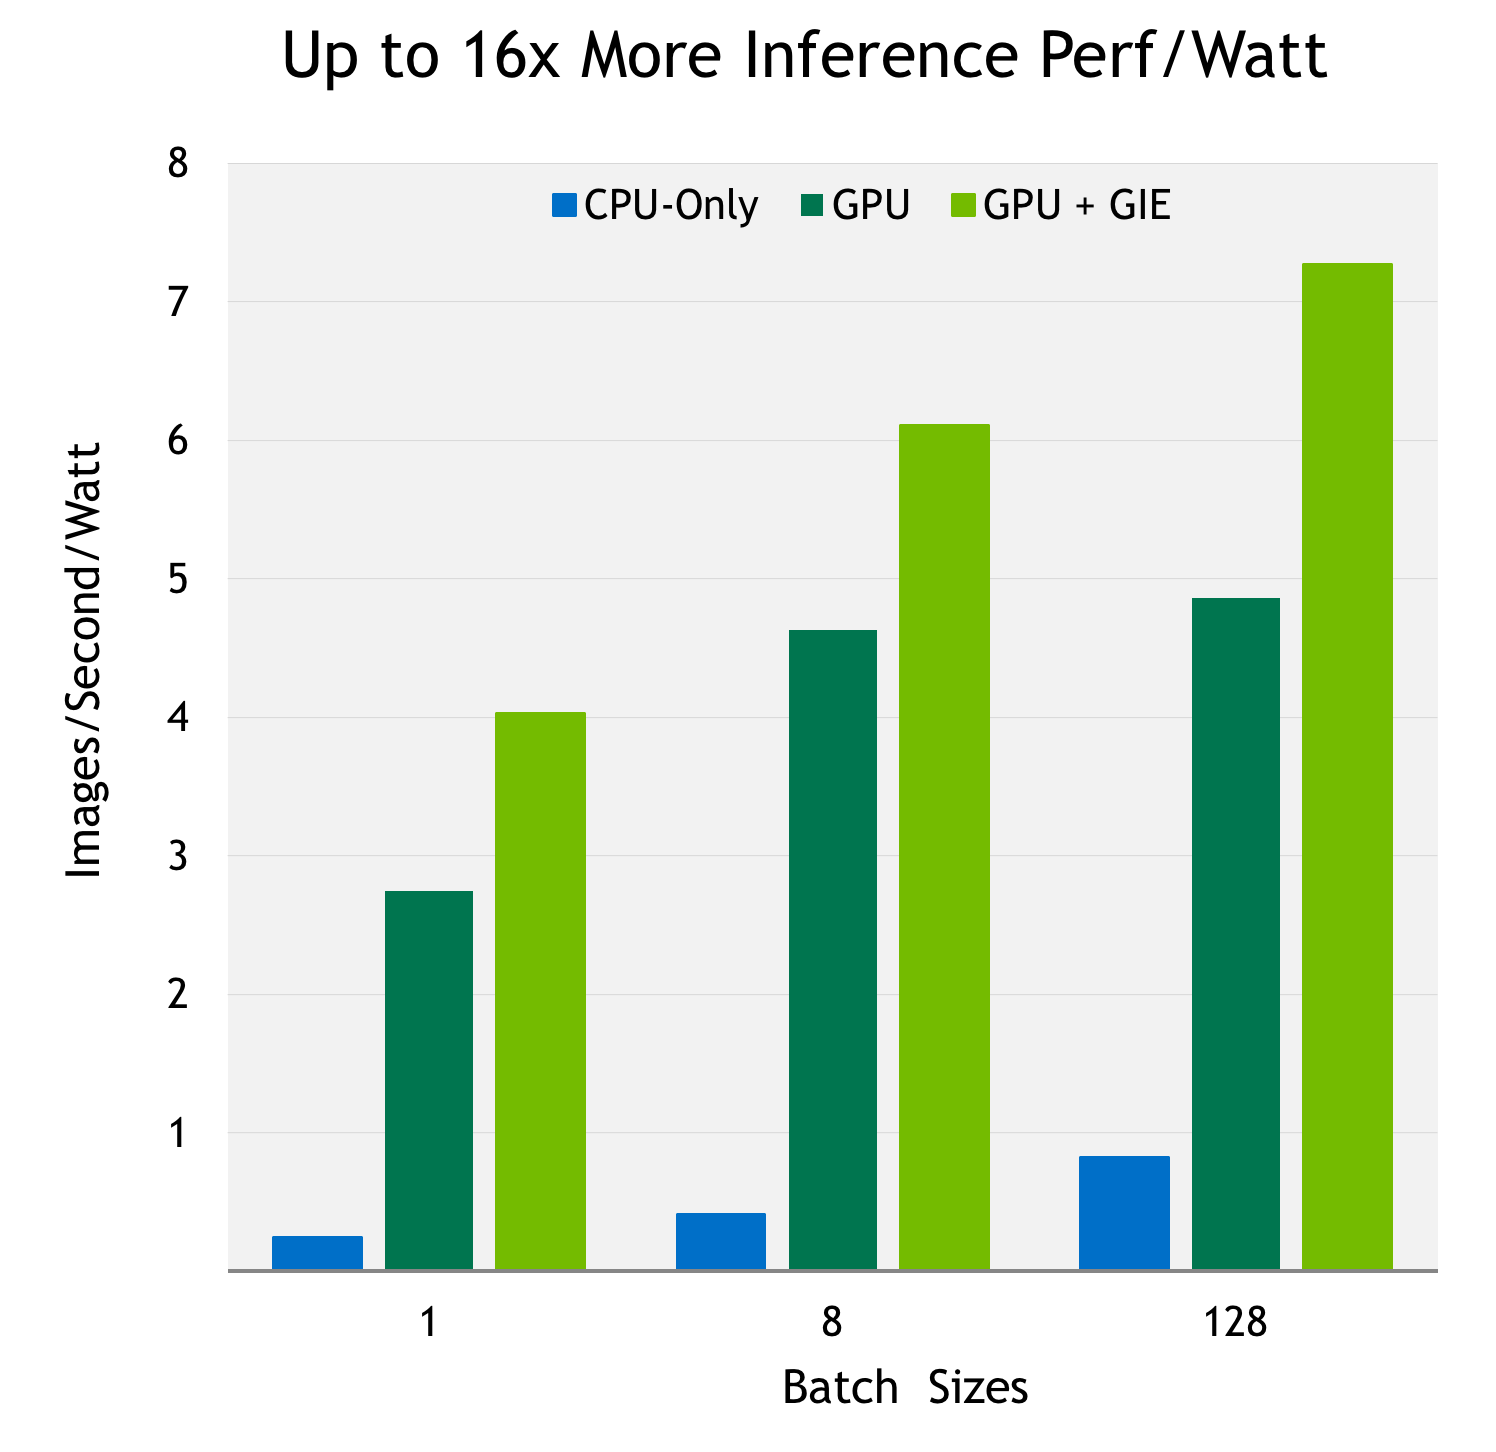
\includegraphics[scale = 0.15]{software1}
    \caption{}
\end{figure}
\begin{figure}
    \centering
    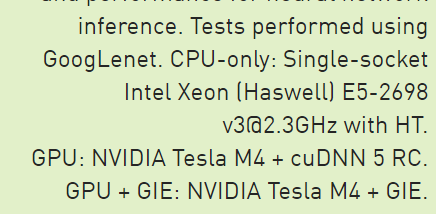
\includegraphics[scale = 0.15]{software2}
    \caption{}
\end{figure}
The graph shows the advantage GPUs provide for training deep learning models.

\subsubsection{Packages}
For my project I have considered using packages to aid the learning process such as Theano. Theano is a CPU and GPU mathematical compiler that outperforms other tools. Theano includes tools for manipulating and optimising graphs representing mathematical functions. An example is the sigmoid function that is used heavily in machine learning. Theano’s optimisation also includes the elimination of duplicates or unnecessary computations therefore increasing the numerical stability as well as increasing speed.  The graph representation allows the user to quickly prototype machine learning models as the differentiation of the function does not have to be calculated in algorithms such as backpropagation. This reduces the amount of code that has to be executed. Theano also uses CUDA to define a class of n-dimensional arrays located in GPU memory with Python bindings. This speeds up the number of operations that are performed per second. Theano can also leverage multi-core CPU architectures to allow for parallelisation on both the CPU and the GPU. Some disadvantages of using Theano include the speed of compiling is a lot larger with bigger models. The error messages are also difficult to understand which will make debugging harder. Theano is a quite low level so the learning curve is steeper.
Another package that I could use is Tensorflow. Tensorflow has a flexible architecture and can be deployed on more than one GPU or CPU. As well as this it shares all the features that Theano has. The reason I am not using it is because it is very high level and does not give you enough control at the base layer.

\subsection{Objectives}
The aim of this project is to be able to make predictions on the price of a stock given historic data of the stock.
\\
\subsubsection{General Objectives}
\\
Data processing
\begin{enumerate}
    \item Must be able to accept a CSV file as an input
    \item Must normalise the data set
\end{enumerate}

Prediction
\begin{enumerate}
    \item Must pass the data through a variable selection block
    \item Must pass the data through an LSTM encoder
    \item Must pass the data through a series of GRNs
    \item Must implement multi head attention
    \item Must return quantile forecasts for the following 5 days
\end{enumerate}

Forecast processing
\begin{enumerate}
    \item Must decide whether to recommend a sell, short or buy
    \item  Must calculate the confidence level of the forecast
\end{enumerate}

User interface
\begin{enumerate}
    \item Must display the forecast along with a confidence level
    \item Must give recommendations for buying, shorting or selling
    \item Consider giving alerts to help the user
\end{enumerate}

\subsubsection{Specific objectives}

Gated Residual network
\begin{enumerate}
    \item Must have a dense network
    \item Must have an exponential linear unit
    \item Must have layer normalisation
    \item Must have a residual connection between the input and output
\end{enumerate}
Variable Selection block
\begin{enumerate}
    \item Must have three GRNs
    \item Must have a GRN with a softmax function
    \item Must calculate the tensor product of the three GRNs
\end{enumerate}
LSTM encoder-decoder
\begin{enumerate}
    \item Must have an encoder model
    \item Must have a decoder model
    \item Must have a dense block
\end{enumerate}
Multi-head attention
\begin{enumerate}
    \item Must take the embedding size, the query size and attention heads as an input
    \item Must have input embedding and position encoding layers to produce a matrix of shape
    \item The matrix must be fed to the query, key and value of the first encoder in the stack
    \item The input must be passed through linear layers to produce the Q, K and V matrices
    \item The data must get split across the attention heads
    \item The Q, K and V matrices must be reshaped
    \item An attention score must be computed for each head
    \item The attention scores must be merged together
\end{enumerate}



\clearpage
\section{Documented Design}
\subsubsection{Heirarchy Diagram}
The project can be split into 3 main sections: data preprocessing, the temporal fusion transformer model and the quantile forecasts.
\begin{figure}[ht]
    \centering
    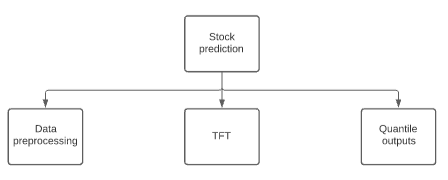
\includegraphics[scale = 0.6]{hd1}
    \caption{}
\end{figure}
Data processing can also be split into 3 parts: Processing, normalisation and adding time embeddings.
\begin{figure}[ht]
    \centering
    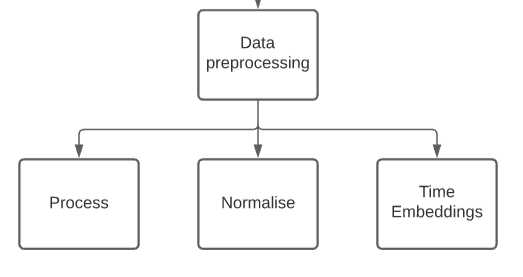
\includegraphics[scale = 0.6]{hd2}
    \caption{}
\end{figure}
Below is a structure diagram of the Temporal Fusion Transformer. It is split into 4 sections: Gated Blocks, LSTM, Variable Selection Network and Multi-head Attention. Each of those sections are further subdivided into the different types of that object.
\begin{figure}[ht]
    \centering
    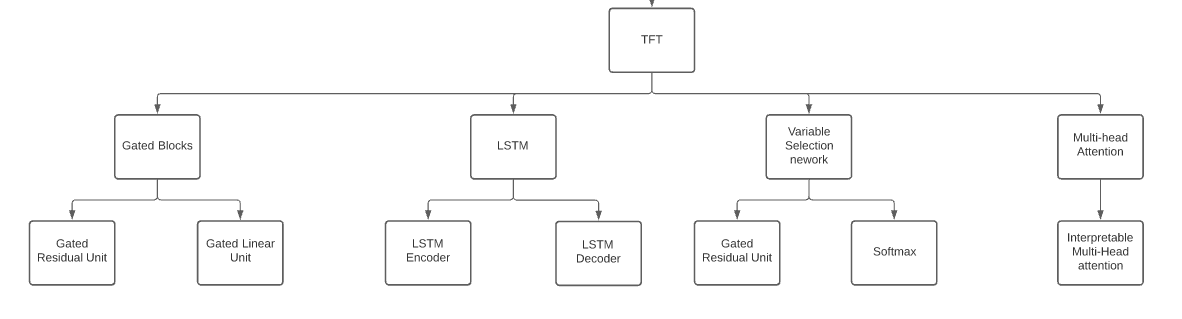
\includegraphics[scale = 0.35]{hd3}
    \caption{}
\end{figure}
The Quantile outputs are split into functions that are used in the main TFT model, layer normalisation, GRU and GLU. These together will form the forecasts at the end.
\begin{figure}[ht]
    \centering
    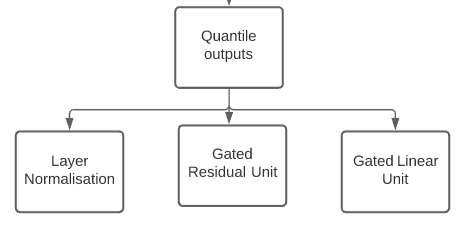
\includegraphics[scale = 0.4]{hd4}
    \caption{}
\end{figure}
The Gated Residual unit can be broken up into 3 parts: the dense network, the exponential unit and the addition and normalisation layer.
\begin{figure}[ht]
    \centering
    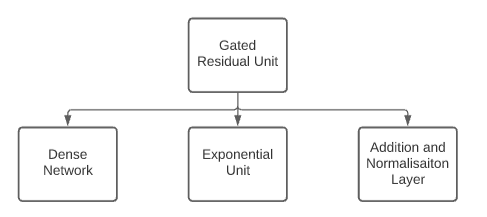
\includegraphics[scale = 0.4]{hd5}
    \caption{}
\end{figure}
This figure shows an overview of the Data Preprocessing. This part of the program will ensure that all the data is fit to be fed to the model and will convert the values into a form that is best for the machine learning module(TFT). This process includes removing all null values, creating the appropriate datasets, vectorising them, adding time embeddings and then finally splitting the datasets into batches.
Removing null values will ensure that sudden spikes in the data do not add a bias to the model. A spike will have a big derivative and might cause the wrong neurons to be activated.
Normalising a dataset will ensure that all the data lies within 0n1. It is required as my data have different ranges. Having all values between the same range is needed to make sure larger values in a dataset don't have a greater importance/bias. This will help speed up the model as the calculations and multiplication will be done with smaller numbers. Rounding is acceptable as we are dealing with a machine learning model and not a statistical learning model. Rounding will not have a significant impact on the overall accuracy.
The dataset has to be split into 3 parts: the training dataset, the validation dataset and the testing dataset. The split will be roughly 80:5:15. It is important to make sure that the training data is not used when testing as this will give us an hyperinflated accuracy, making the model seem a lot better than it actually is.
The datasets then have to be vectorised as the model will only take in vectors, matrices or tensors.
Time embeddings are added to the data. This is to help the attention part of the model. Attention works by referring back to the previous data points and so each data point has to be given a time stamp/embedding.
The positional encoder will assign data points a value to determine their position in the dataset. This is also used to help make sure the attention module works,
The dataset will finally be split up into batches. This is so that I can conduct batch training. This helps the model focus on small sections of the data instead of trying to consider all the data at once. This helps the code be more memory efficient and will lead to a higher accuracy score.

\clearpage
\begin{figure}[ht]
    \centering
    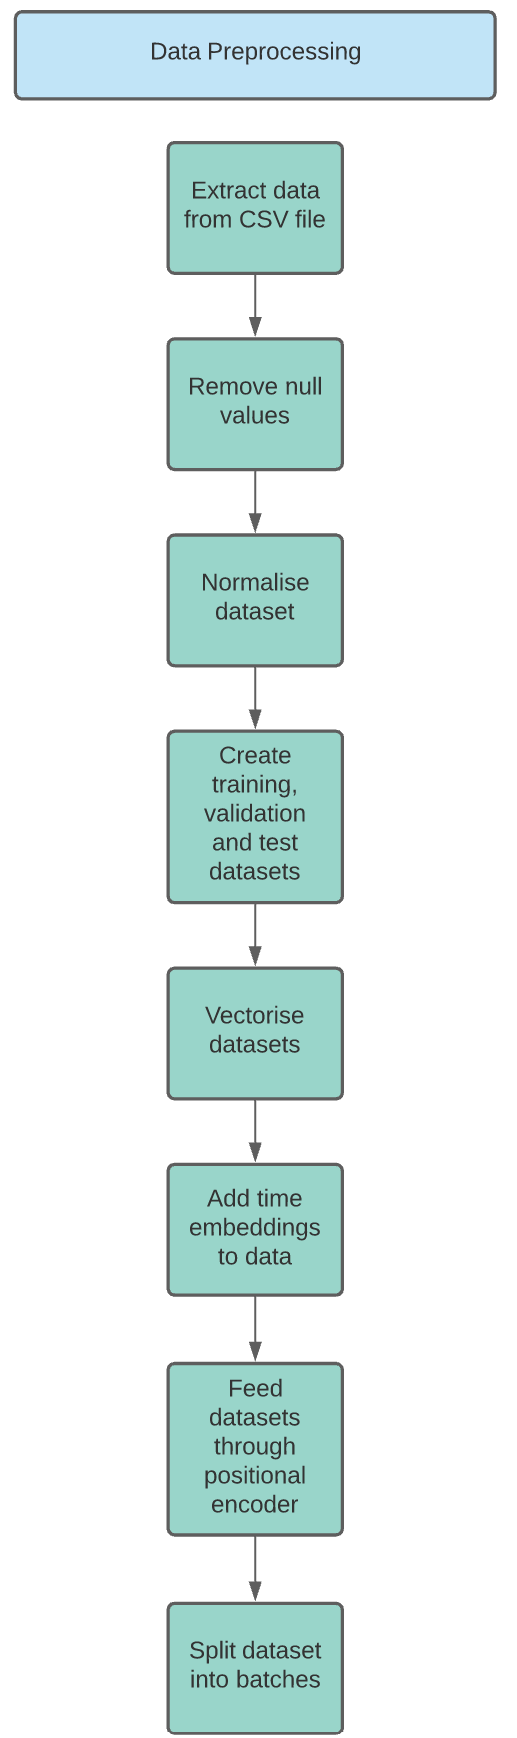
\includegraphics[scale = 0.5]{hd6}
    \caption{}
\end{figure}
The figure above shows how the attention mechanism works. The module takes in 3 input vectors: Query, Key and Value. These are fed into the attention block and an Attention score is calculated using the equation detailed in the analysis section. The multiple linear and attention score blocks represent the number of heads in the attention block.
\begin{figure}[ht]
    \centering
    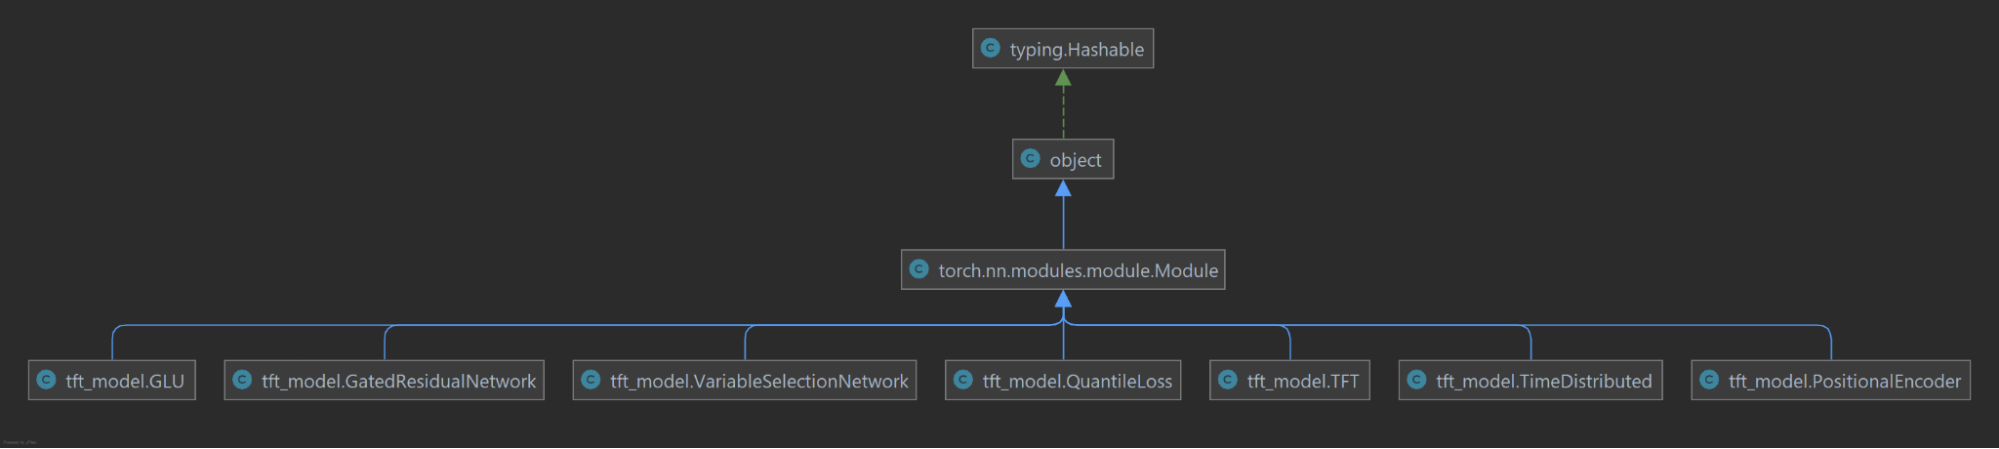
\includegraphics[scale = 0.15]{hd7}
    \caption{}
\end{figure}
Above is a flowchart to show the travel of data in my program. The TFT module starts off with the quantile loss and ends with the output layer.
The logging metric is going to be in the form of a tensorboard. This tracks important data such as the change in loss as the number of epochs increases. I can track and see the change in weights through the neural network. This helps me evaluate the performance of certain blocks in the TFT. The tensorboard will also allow me to compare different initialisation techniques such as truncated and xavier. The most important reason is to find out when to stop training the model. The graph of loss vs epoch can be thought of as a 1x graph for 0x. As the graph starts to level off, the net effect of each epoch decreases. Training a machine learning algorithm is time, space and cost intensive so any effort to reduce the number of epochs has to be taken. Analysing the graph provided by the tensorboard will allow this.
The main part of the machine learning model(TFT) aims to pass the data through many blocks that will analyse the overall trend in the data while observing patterns in the data. The use of LSTMs and Gated Residual Units contain memory blocks that help the neural network consider context. At the start there are encoders and so therefore later on decoders are required. Multihead attention is used later on to use attention to provide further context to the model.

\begin{figure}[ht]
    \centering
    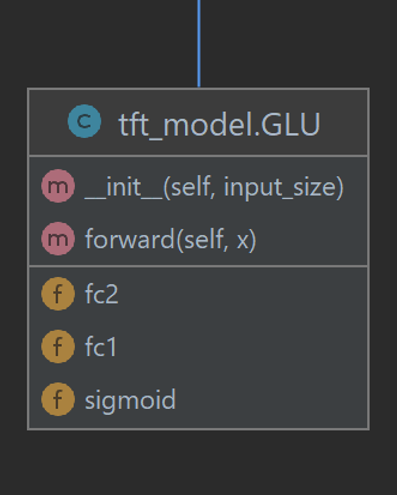
\includegraphics[scale = 0.6]{hd8}
    \caption{}
\end{figure}
\begin{figure}[ht]
    \centering
    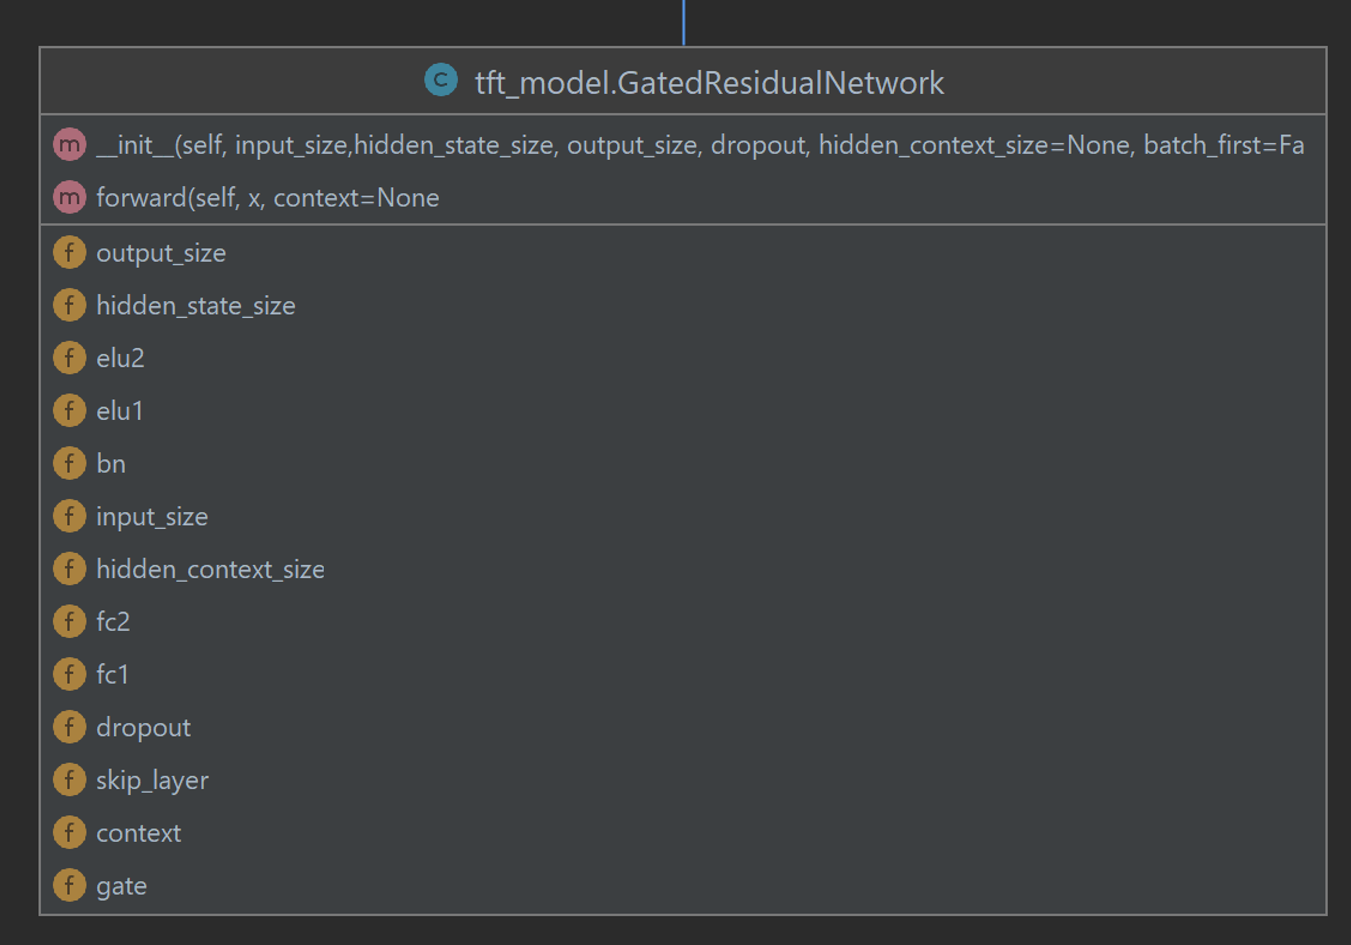
\includegraphics[scale = 0.315]{hd9}
    \caption{}
\end{figure}
\begin{figure}[ht]
    \centering
    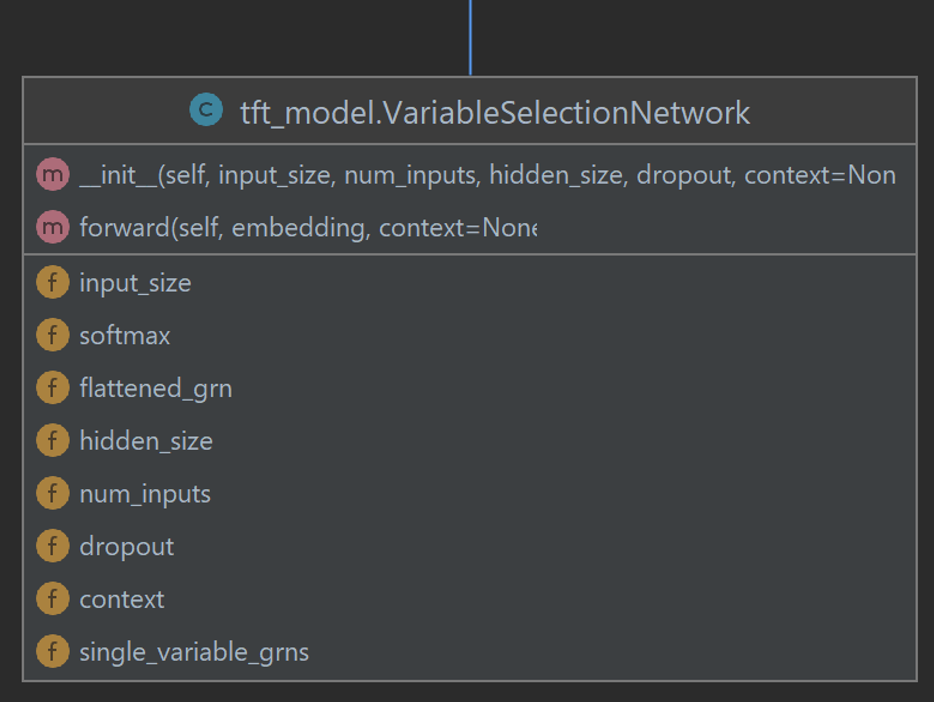
\includegraphics[scale = 0.35]{hd10}
    \caption{}
\end{figure}
\begin{figure}[ht]
    \centering
    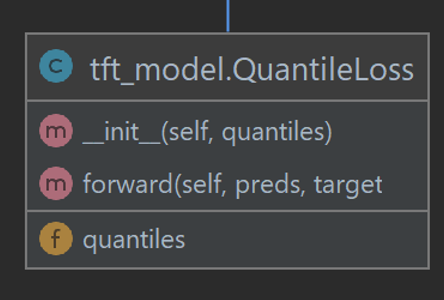
\includegraphics[scale = 0.35]{hd11}
    \caption{}
\end{figure}
\begin{figure}[ht]
    \centering
    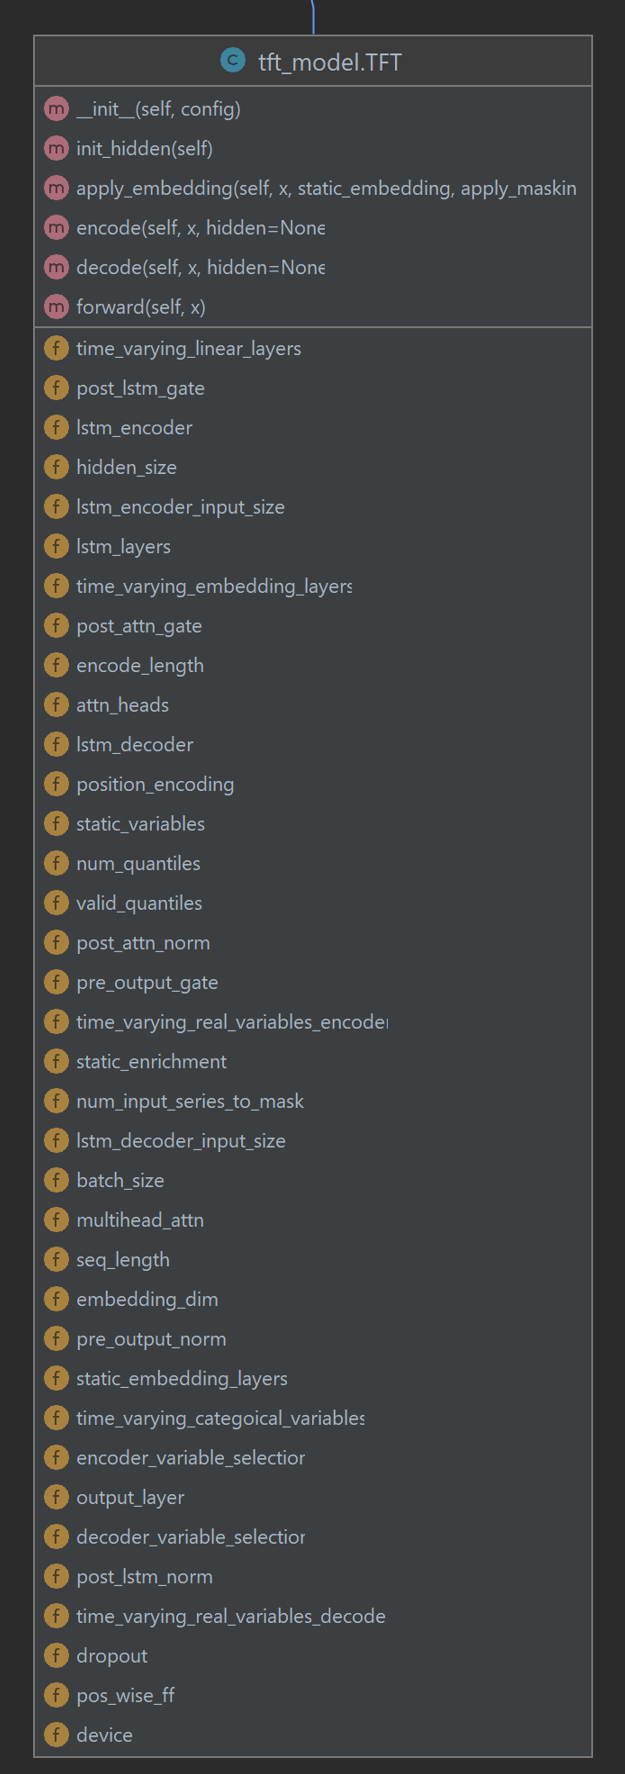
\includegraphics[scale = 0.35]{hd12}
    \caption{}
\end{figure}
\begin{figure}[ht]
    \centering
    \includegraphics[scale = 0.35]{h13}
    \caption{}
\end{figure}
\begin{figure}[ht]
    \centering
    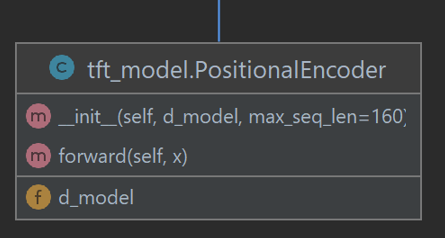
\includegraphics[scale = 0.25]{hd14}
    \caption{}
\end{figure}
\begin{figure}[ht]
    \centering
    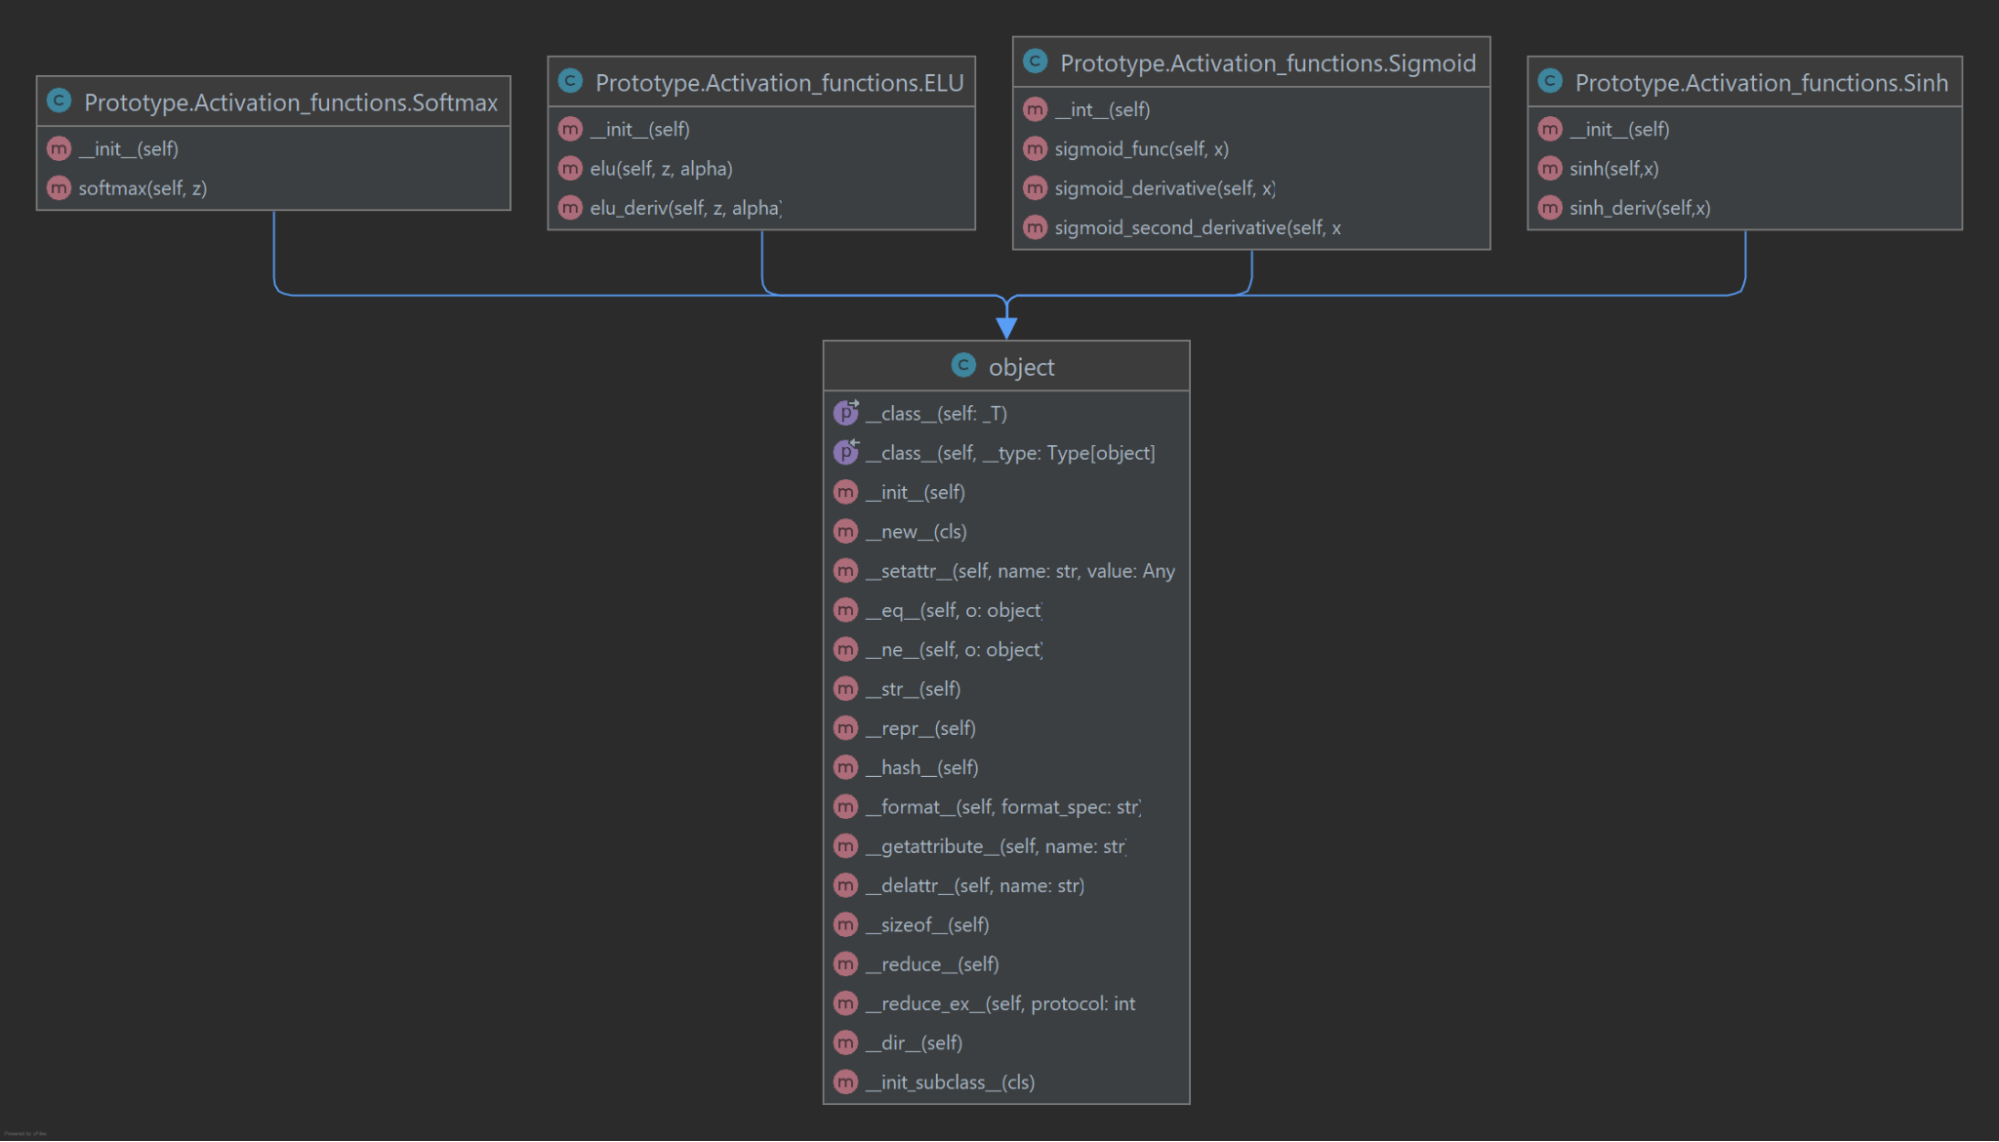
\includegraphics[scale = 0.15]{hd15}
    \caption{}
\end{figure}
\begin{figure}[ht]
    \centering
    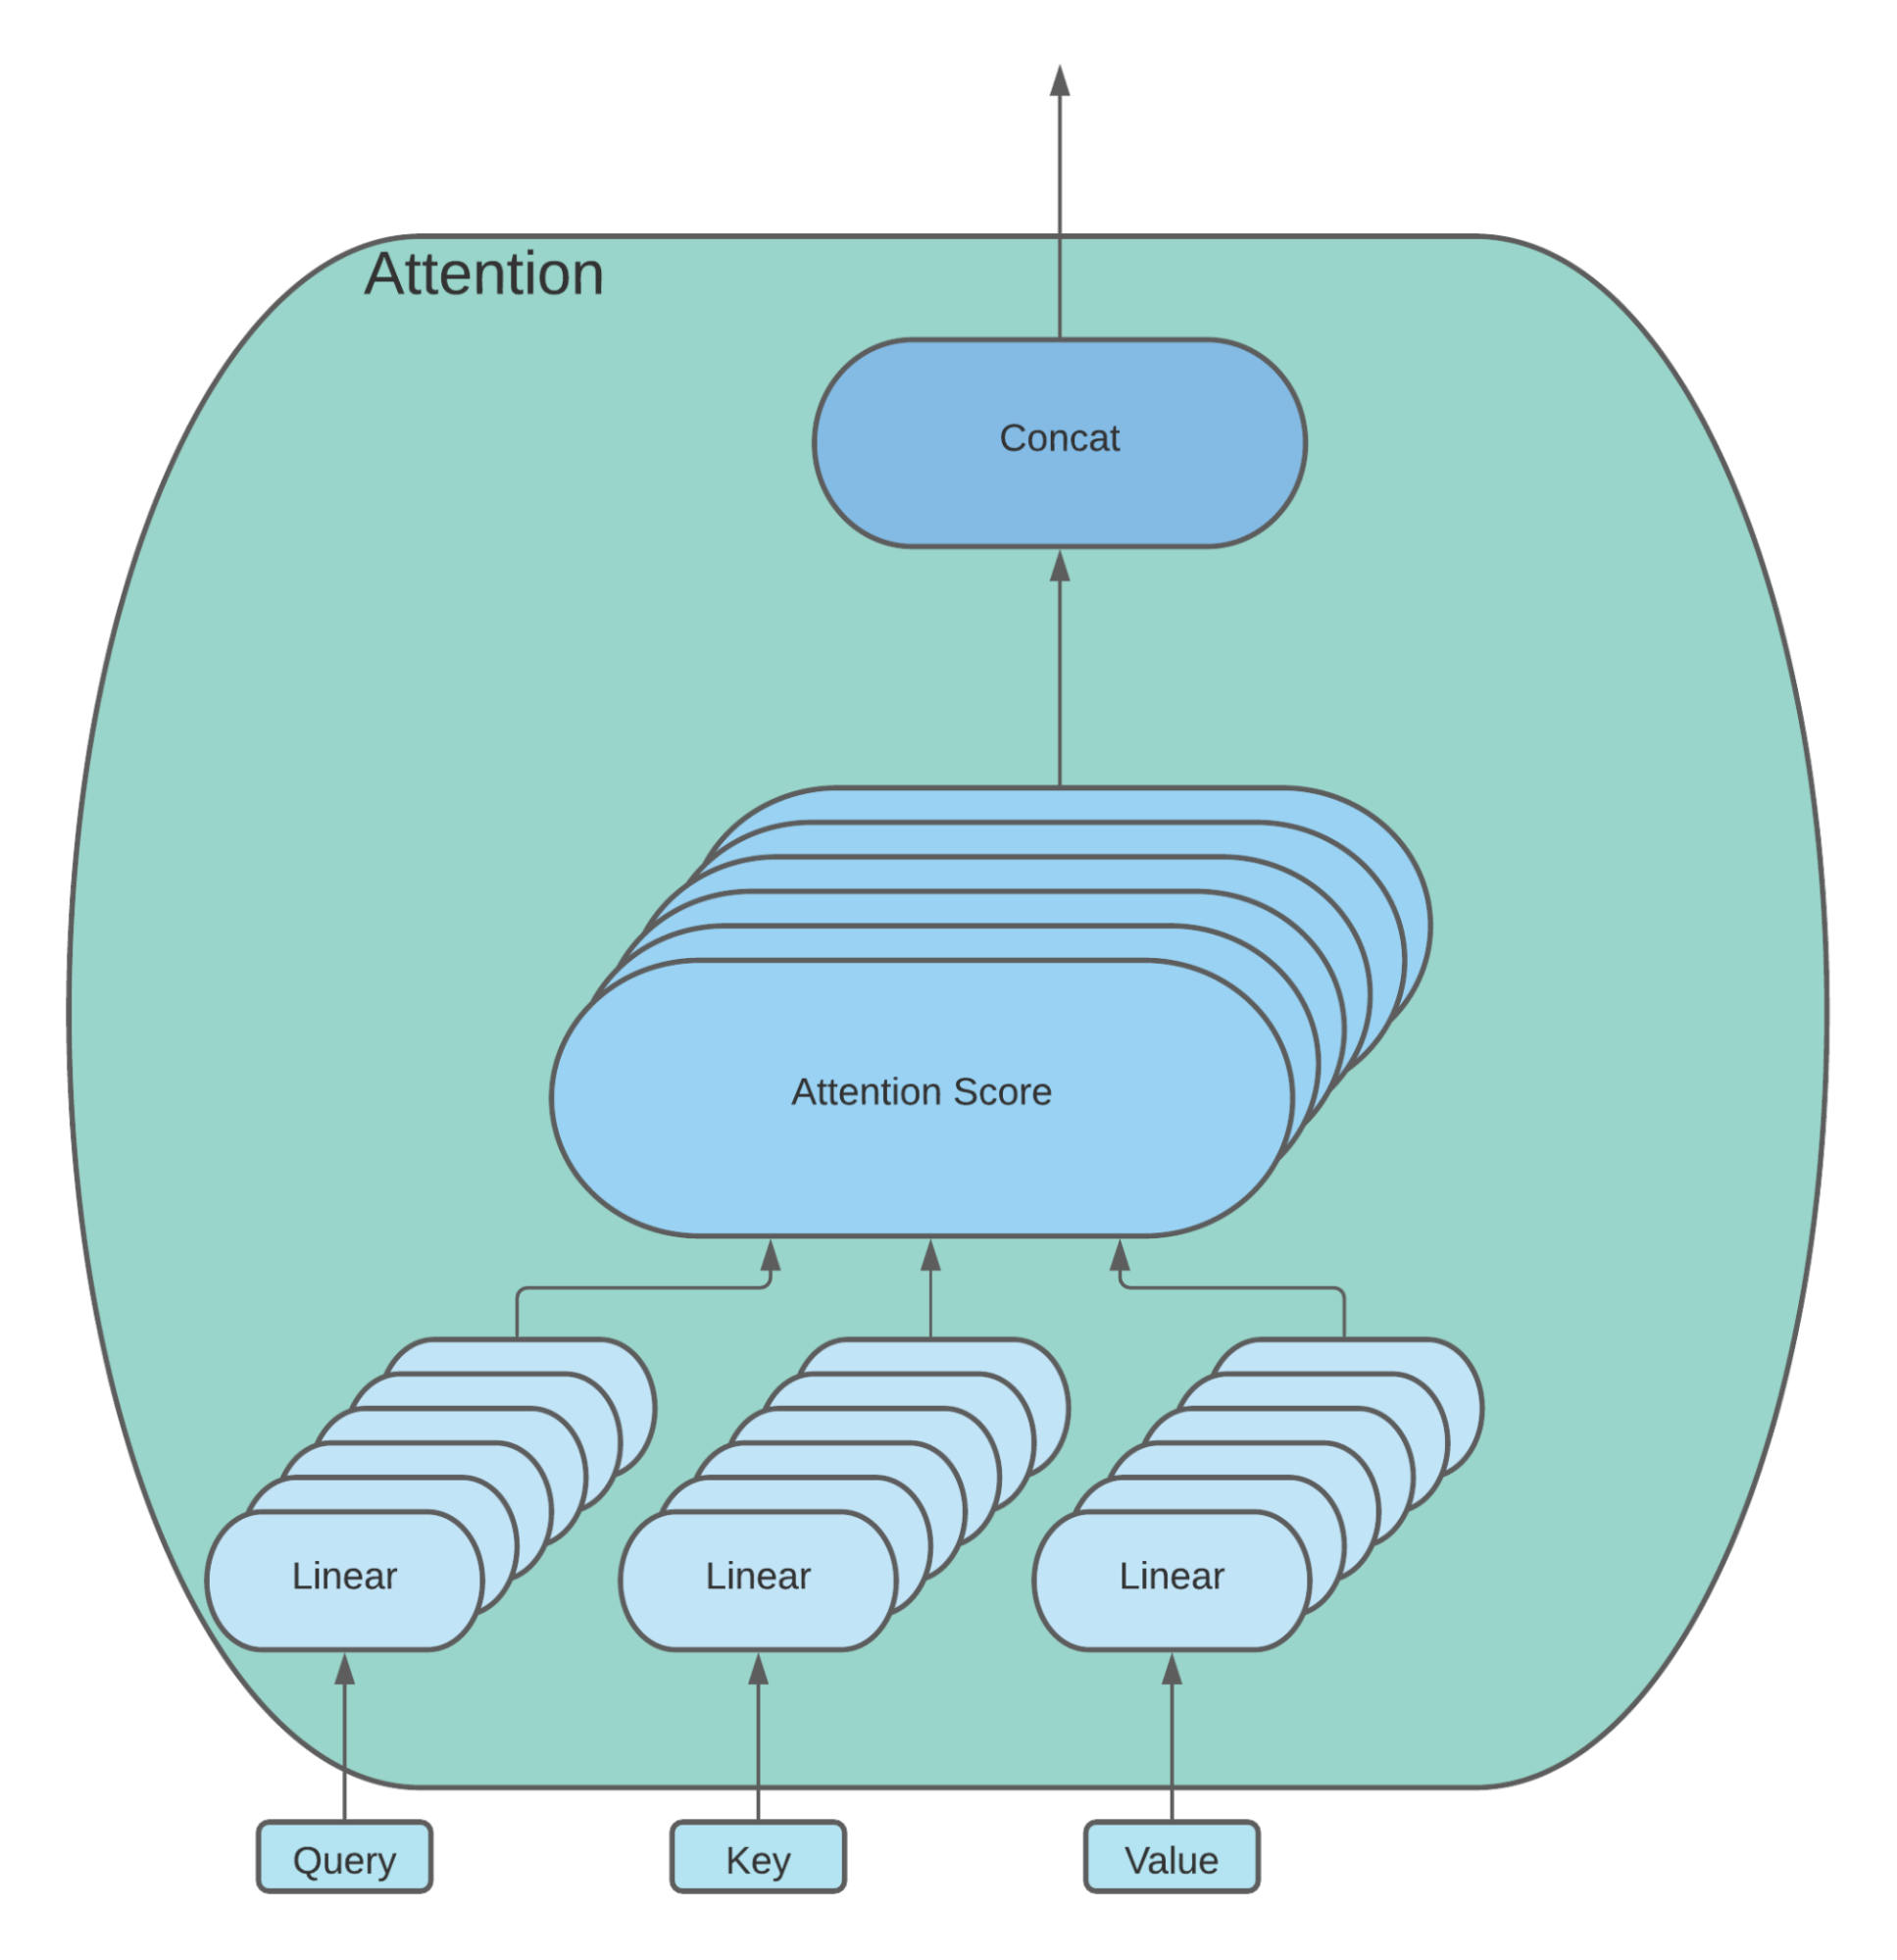
\includegraphics[scale = 0.15]{attention1}
    \caption{}
\end{figure}
\begin{figure}[ht]
    \centering
    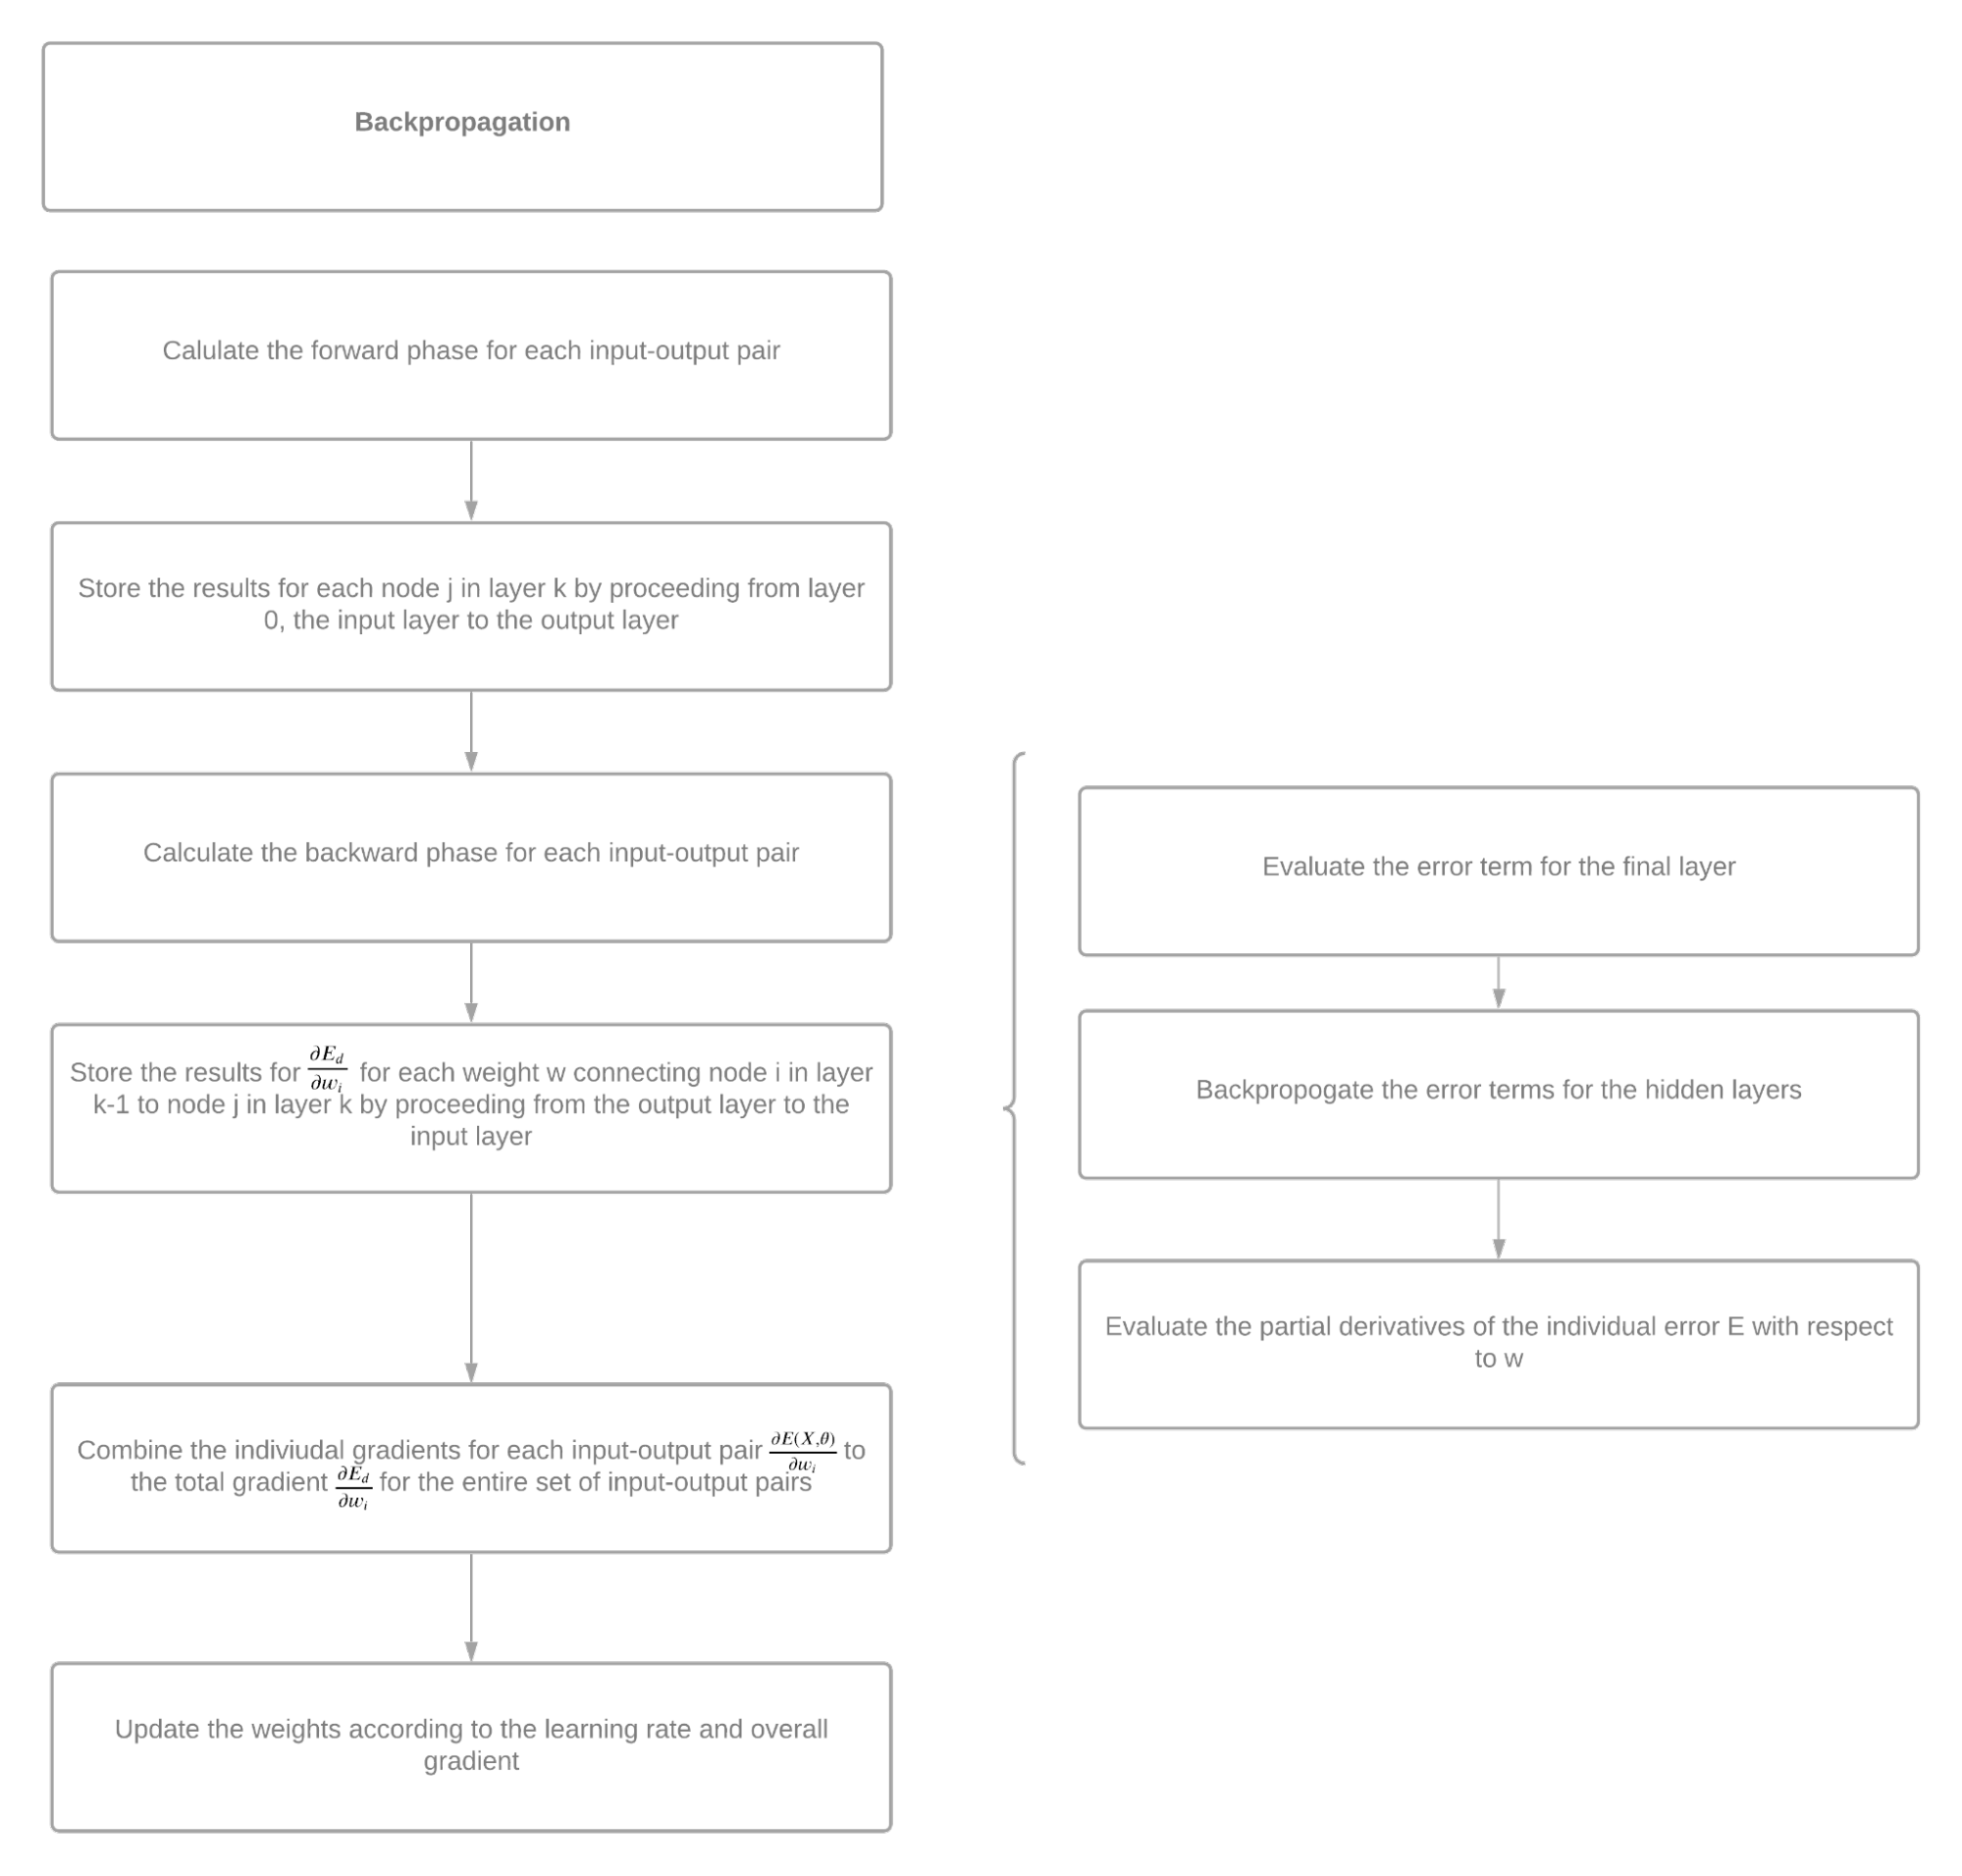
\includegraphics[scale = 0.24]{backprop1}
    \caption{}
\end{figure}
\begin{figure}[ht]
    \centering
    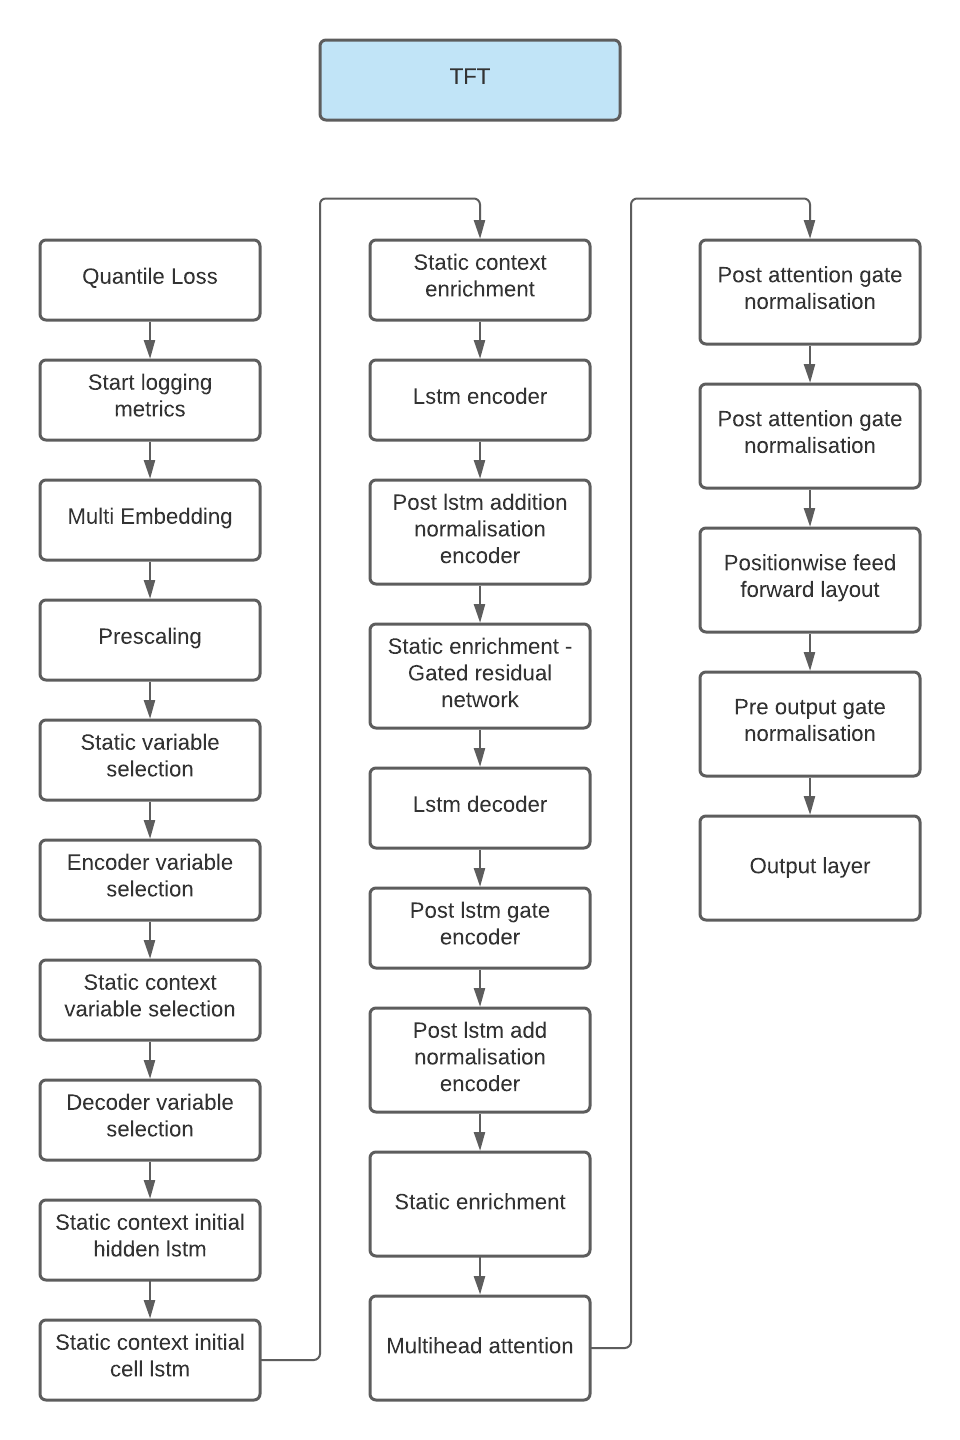
\includegraphics[scale = 0.4]{tft2}
    \caption{}
\end{figure}


\clearpage


The TFT can be modelled using the structure below. This shows the flow of data through one epoch of the network.  Each module has the dimensions, input features, output features, activation functions and learning rate specified.

\begin{lstlisting}
TemporalFusionTransformer(
  (loss): QuantileLoss()
  (logging_metrics): ModuleList(
    (0): SMAPE()
    (1): MAE()
    (2): RMSE()
    (3): MAPE()
  )
  (input_embeddings): MultiEmbedding(
    (embeddings): ModuleDict()
  )
  (prescalers): ModuleDict()
  (static_variable_selection): VariableSelectionNetwork(
    (single_variable_grns): ModuleDict()
    (prescalers): ModuleDict()
    (softmax): Softmax(dim=-1)
  )
  (encoder_variable_selection): VariableSelectionNetwork(
    (single_variable_grns): ModuleDict()
    (prescalers): ModuleDict()
    (softmax): Softmax(dim=-1)
  )
  (decoder_variable_selection): VariableSelectionNetwork(
    (single_variable_grns): ModuleDict()
    (prescalers): ModuleDict()
    (softmax): Softmax(dim=-1)
  )
  (static_context_variable_selection): GatedResidualNetwork(
    (fc1): Linear(in_features=16, out_features=16, bias=True)
    (elu): ELU(alpha=1.0)
    (fc2): Linear(in_features=16, out_features=16, bias=True)
    (gate_norm): GateAddNorm(
      (glu): GatedLinearUnit(
        (dropout): Dropout(p=0.1, inplace=False)
        (fc): Linear(in_features=16, out_features=32, bias=True)
      )
      (add_norm): AddNorm(
        (norm): LayerNorm((16,), eps=1e-05, elementwise_affine=True)
      )
    )
  )
  (static_context_initial_hidden_lstm): GatedResidualNetwork(
    (fc1): Linear(in_features=16, out_features=16, bias=True)
    (elu): ELU(alpha=1.0)
    (fc2): Linear(in_features=16, out_features=16, bias=True)
    (gate_norm): GateAddNorm(
      (glu): GatedLinearUnit(
        (dropout): Dropout(p=0.1, inplace=False)
        (fc): Linear(in_features=16, out_features=32, bias=True)
      )
      (add_norm): AddNorm(
        (norm): LayerNorm((16,), eps=1e-05, elementwise_affine=True)
      )
    )
  )
  (static_context_initial_cell_lstm): GatedResidualNetwork(
    (fc1): Linear(in_features=16, out_features=16, bias=True)
    (elu): ELU(alpha=1.0)
    (fc2): Linear(in_features=16, out_features=16, bias=True)
    (gate_norm): GateAddNorm(
      (glu): GatedLinearUnit(
        (dropout): Dropout(p=0.1, inplace=False)
        (fc): Linear(in_features=16, out_features=32, bias=True)
      )
      (add_norm): AddNorm(
        (norm): LayerNorm((16,), eps=1e-05, elementwise_affine=True)
      )
    )
  )
  (static_context_enrichment): GatedResidualNetwork(
    (fc1): Linear(in_features=16, out_features=16, bias=True)
    (elu): ELU(alpha=1.0)
    (fc2): Linear(in_features=16, out_features=16, bias=True)
    (gate_norm): GateAddNorm(
      (glu): GatedLinearUnit(
        (dropout): Dropout(p=0.1, inplace=False)
        (fc): Linear(in_features=16, out_features=32, bias=True)
      )
      (add_norm): AddNorm(
        (norm): LayerNorm((16,), eps=1e-05, elementwise_affine=True)
      )
    )
  )
  (lstm_encoder): LSTM(16, 16, batch_first=True)
  (lstm_decoder): LSTM(16, 16, batch_first=True)
  (post_lstm_gate_encoder): GatedLinearUnit(
    (dropout): Dropout(p=0.1, inplace=False)
    (fc): Linear(in_features=16, out_features=32, bias=True)
  )
  (post_lstm_gate_decoder): GatedLinearUnit(
    (dropout): Dropout(p=0.1, inplace=False)
    (fc): Linear(in_features=16, out_features=32, bias=True)
  )
  (post_lstm_add_norm_encoder): AddNorm(
    (norm): LayerNorm((16,), eps=1e-05, elementwise_affine=True)
  )
  (post_lstm_add_norm_decoder): AddNorm(
    (norm): LayerNorm((16,), eps=1e-05, elementwise_affine=True)
  )
  (static_enrichment): GatedResidualNetwork(
    (fc1): Linear(in_features=16, out_features=16, bias=True)
    (elu): ELU(alpha=1.0)
    (context): Linear(in_features=16, out_features=16, bias=False)
    (fc2): Linear(in_features=16, out_features=16, bias=True)
    (gate_norm): GateAddNorm(
      (glu): GatedLinearUnit(
        (dropout): Dropout(p=0.1, inplace=False)
        (fc): Linear(in_features=16, out_features=32, bias=True)
      )
      (add_norm): AddNorm(
        (norm): LayerNorm((16,), eps=1e-05, elementwise_affine=True)
      )
    )
  )
  (multihead_attn): InterpretableMultiHeadAttention(
    (dropout): Dropout(p=0.1, inplace=False)
    (v_layer): Linear(in_features=1, out_features=4, bias=True)
    (q_layers): ModuleList(
      (0): Linear(in_features=16, out_features=4, bias=True)
      (1): Linear(in_features=16, out_features=4, bias=True)
      (2): Linear(in_features=16, out_features=4, bias=True)
      (3): Linear(in_features=16, out_features=4, bias=True)
    )
    (k_layers): ModuleList(
      (0): Linear(in_features=16, out_features=4, bias=True)
      (1): Linear(in_features=16, out_features=4, bias=True)
      (2): Linear(in_features=16, out_features=4, bias=True)
      (3): Linear(in_features=16, out_features=4, bias=True)
    )
    (attention): ScaledDotProductAttention(
      (softmax): Softmax(dim=2)
    )
    (w_h): Linear(in_features=4, out_features=16, bias=False)
  )
  (post_attn_gate_norm): GateAddNorm(
    (glu): GatedLinearUnit(
      (dropout): Dropout(p=0.1, inplace=False)
      (fc): Linear(in_features=16, out_features=32, bias=True)
    )
    (add_norm): AddNorm(
      (norm): LayerNorm((16,), eps=1e-05, elementwise_affine=True)
    )
  )
  (pos_wise_ff): GatedResidualNetwork(
    (fc1): Linear(in_features=16, out_features=16, bias=True)
    (elu): ELU(alpha=1.0)
    (fc2): Linear(in_features=16, out_features=16, bias=True)
    (gate_norm): GateAddNorm(
      (glu): GatedLinearUnit(
        (dropout): Dropout(p=0.1, inplace=False)
        (fc): Linear(in_features=16, out_features=32, bias=True)
      )
      (add_norm): AddNorm(
        (norm): LayerNorm((16,), eps=1e-05, elementwise_affine=True)
      )
    )
  )
  (pre_output_gate_norm): GateAddNorm(
    (glu): GatedLinearUnit(
      (fc): Linear(in_features=16, out_features=32, bias=True)
    )
    (add_norm): AddNorm(
      (norm): LayerNorm((16,), eps=1e-05, elementwise_affine=True)
    )
  )
  (output_layer): Linear(in_features=16, out_features=7, bias=True)
)


\end{lstlisting}




\subsection{Explaining nn.module}
Below is the pseduocode for the module followed by the python code.
\begin{algorithm}
\caption{Linear Neural Network}
\begin{algorithmic}[1]
\STATE $Convolution1 \leftarrow ConvertTo2d(x,y,z)$
\STATE $Convolution2 \leftarrow ConvertTo2d(u,v,w)$
\STATE $y \leftarrow Wx + b$
\STATE $fc1 \leftarrow LinearTranformation()$ \Comment{Apply a linear transformation}
\STATE $fc2 \leftarrow LinearTranformation()$
\STATE $fc3 \leftarrow LinearTranformation()$
\STATE $x \leftarrow Apply2DPool(RELU(Convolution1(x)), (2, 2))$
\STATE $x \leftarrow Apply2DPool(RELU(Convolution1(x)),2 )$
\STATE $RELU(fc1(x))$
\STATE $RELU(fc2(x))$
\RETURN $x$
\end{algorithmic}
\end{algorithm}


\begin{lstlisting}
import math
import numpy as np

#Vanilla Neural Network from scratch
class Layer_Dense:
    def __init__(self, n_inputs, n_neurons):
        self.weights = 0.10 * np.random.randn(n_inputs, n_neurons)
        self.biases = np.zeros((1, n_neurons))

   def forward(self, inputs):
        self.output = np.dot(inputs, self.weights) + self.biases


#Activation Functions
class Activation_ReLU:
    def forward(self, inputs):
        self.output = np.maximum(0, inputs)

class Activation_sigmoid:
    def forward(self, inputs):
        self.output = np.exp()

layer1 = Layer_Dense(2,5)
activation1 = Activation_ReLU()
layer2 = Layer_Dense(2,5)
activation2 = Activation_sigmoid()
layer1.forward(X)
print(layer1.forward(x))


#using nn.module
class Net(nn.Module):

    def __init__(self):
        super(Net, self).__init__()
        # 1 input image channel, 6 output channels, 5x5 square convolution kernel
        self.conv1 = nn.Conv2d(1, 6, 5)
        self.conv2 = nn.Conv2d(6, 16, 5)

        # an affine operation: y = Wx + b
        self.fc1 = nn.Linear(16 * 5 * 5, 120)
        self.fc2 = nn.Linear(120, 84)
        self.fc3 = nn.Linear(84, 10)

    def forward(self, x):
        # Max pooling over a (2, 2) window
        x = F.max_pool2d(F.relu(self.conv1(x)), (2, 2))

        # 2 is ame as (2, 2)
        x = F.max_pool2d(F.relu(self.conv2(x)), 2)

        x = x.view(-1, self.num_flat_features(x))
        x = F.relu(self.fc1(x))
        x = F.relu(self.fc2(x))
        x = self.fc3(x)

        return x

    def num_flat_features(self, x):
        size = x.size()[1:]  # all dimensions except the batch dimension
        num_features = 1
        for s in size:       # Get the products
            num_features *= s
        return num_features
\end{lstlisting}

\clearpage

\subsection{Positional Encoding}
One of the reasons for using sine and cosine functions is that they are periodic and so whether the model is learning on a sequence of length 5, or of length 500, the encodings will always have the same range ([-1, 1]).  Positional embeddings are added to the original embeddings to retain all the positional information. Each vector will be parametrized and the stack row-wise to form a learnable positional embedding table.
\\
%\begin{equation}
$PE_{pos+k}$ is some matrix which depends on k times PE_{pos}\\
$$PE_{pos+k, 2i} = sin(\frac{pos}{a}+\frac{k}{a})$$\\
$$ =sin(\frac{pos}{a})cos(\frac{k}{a})+sin(\frac{k}{a})cos(\frac{pos}{a})$$\\
$$ =(PE_{pos,2i+1})U+(PE_{pos,2i})V$$\\
$$ =(PE_{pos,2i},PE_{pos,2i+1})(V,U)$$\\
%\end{equation}

\begin{algorithm}
\caption{Positional Encoder}
\begin{algorithmic}
\For{pos in  0 $\leftarrow$ maximum sequence length}
    \State{compute V$\times$PE(pos,2i)}
    \State{computeW$\times$PE(pos,2i)}
    \State{compute V$\times$PE(pos,2i+1)}
    \State{compute W$\times$PE(pos,2i+1)}
\EndFor
\end{algorithmic}
\end{algorithm}


\\Python code:


\begin{lstlisting}
#positional encoding
import torch
import math


class PositionalEncoder(torch.nn.Module):
    def __init__(self, d_model, max_len=5000):
        self.d_model = d_model # the size of the embedding vectors
        self.max_len = max_len
        # Compute the positional encodings once in log space complexity
        pe = torch.zeros(max_len, d_model)
        position = torch.arange(0, max_len).unsqueeze(1)
        div_term = torch.exp(torch.arange(0, d_model, 2) *
                             -(math.log(10000.0) / d_model))
        pe[:, 0::2] = torch.sin(position * div_term)
        pe[:, 1::2] = torch.cos(position * div_term)
        pe = pe.unsqueeze(0)
        self.register_buffer('pe', pe)

    def forward(self, x):
        x = x + self.pe[:, :x.size(1)]
        return x

    def get_embedding(self, x):
        x = x + self.pe[:, :x.size(1)]
        return x

    def get_embedding_layer(self):
        return torch.nn.Embedding(self.max_len, self.d_model)

\end{lstlisting}
\clearpage
\subsection{Backpropagation}
The formula for the backpropagation algorithm has been proven earlier in the analysis. Below is a reminder of the mathematical definition along with a flowchart and pseudocode.

Partial derivatives:
$$\frac{\partial{E_d}}{\partial{w_j^k}} = \delta_j^k o_i^{k-1}$$
Final layer's error term:
$$\delta_1^m = g_o'(a_1^m)(\hat{y_d-y_d})$$
Hidden layers' error terms:
$$\delta_j^k = g''(a_j^k)\sum_{L=1}^{r^{k+1}}w^{k+1}_jL\delta_l^{k+1}$$
Computing the partial derivatives for each input-output pair:
    $$\frac{\partial{E(X,\theta)}}{\partial{w_ij^k}}= \frac{1}{N}\sum_{d=1}^{N}\frac{\delta}{\delta w_ij^k}(\frac{1}{2}(\hat{y_d}-y_d)^2)$$
    $$ = \frac{1}{N}\sum_{d=1}^{N}\frac{\partial{E_d}}{\partial{w_ij^k}}$$
Updating weights:
$$ \Delta w_ij^k = -\alpha \frac{\partial{E(X,\theta)}}{\partial{w_ij^k}}$$
\begin{algorithm}
\caption{Backpropagation}
\begin{algorithmic}[1]
\Function{Backpropagation}{inputs, expected, output}
    \State {deltas $\leftarrow$delta inputs}
    \Repeat{}
    \For{i in deltas}
        \State{error $\leftarrow$ expected[i] - output
        deltas[i]$\leftarrow$ error$\times$sigmoid}
    \For{j in hidden layers}
        \For{k in hidden weights}
           \State{delta weights$\leftarrow$ weight[j] $\times$ outputdeltas[k]}
            \State{deltaweights$\times$ learning rate}
\EndFunction
\end{algorithmic}
\end{algorithm}
\clearpage
\begin{lstlisting}
# backpropagate() takes as input, the patterns entered, the target values and the obtained values.
# Based on these values, it adjusts the weights so as to balance out the error.
# Also, now we have M, N for momentum and learning factors respectively.
def backpropagate(self, inputs, expected, output, N=0.5, M=0.1):
	# We introduce a new matrix called the deltas (error) for the two layers output and hidden layer respectively.
	output_deltas = [0.0]*self.no
	for k in range(self.no):
		# Error is equal to (Target value - Output value)
		error = expected[k] - output[k]
		output_deltas[k]=error*dsigmoid(self.ao[k])

	# Change weights of hidden to output layer accordingly.
	for j in range(self.nh):
		for k in range(self.no):
			delta_weight = self.ah[j] * output_deltas[k]
			self.who[j][k]+= M*self.cho[j][k] + N*delta_weight
			self.cho[j][k]=delta_weight

	# Now for the hidden layer.
	hidden_deltas = [0.0]*self.nh
	for j in range(self.nh):
		# Error as given by formule is equal to the sum of (Weight from each node in hidden layer times output delta of output node)
		# Hence delta for hidden layer = sum (self.who[j][k]*output_deltas[k])
		error=0.0
		for k in range(self.no):
			error+=self.who[j][k] * output_deltas[k]
		# now, change in node weight is given by dsigmoid() of activation of each hidden node times the error.
		hidden_deltas[j]= error * dsigmoid(self.ah[j])

	for i in range(self.ni):
		for j in range(self.nh):
			delta_weight = hidden_deltas[j] * self.ai[i]
			self.wih[i][j]+= M*self.cih[i][j] + N*delta_weight
			self.cih[i][j]=delta_weight
\end{lstlisting}
\clearpage
\subsection{Dense Network}
This is the fundamental block, similar to the nn.module. This is another vanilla
neural network.

\begin{lstlisting}
class Dense_Network:
    def __init__(self, input_shape, output_shape, activation, weights, biases):
        self.input_shape = input_shape
        self.output_shape = output_shape
        self.activation = activation
        self.weights = weights
        self.biases = biases
        self.output = None
        self.input = None

    def forward_pass(self, input):
        self.input = input
        self.output = np.dot(self.input, self.weights) + self.biases
        self.output = self.activation(self.output)
        return self.output

    def backward_pass(self, error):
        self.error = error
        self.error = self.error * self.activation(self.output, derivative=True)
        self.weights_error = np.dot(self.input.T, self.error)
        self.biases_error = np.sum(self.error, axis=0)
        return self.error

    def update_weights(self, learning_rate):
        self.weights = self.weights - learning_rate * self.weights_error
        self.biases = self.biases - learning_rate * self.biases_error

    def get_weights(self):
        return self.weights


\end{lstlisting}

\clearpage


\subsection{Weight Initialisation}
\subsubsection{Theory}
Weight initialisation is essential when training a neural network. This process prevents
activation functions from exploding or vanishing when executing a forward pass. If the weights are too large, the variance of the input data tends to increase rapidly with each pass, eventually
getting to a point where the derivative tends to 0. This is why it is important to initialise the network with the right weights. The range in which the it is initialised will be governed using a technique called Xavier initialisation.\\
Xavier works by assigning the weights from a Gaussian distribution
Consider a distrubtion with mean 0 and some finite variance as well as a linear neuron: $$y = w_1x_1 + w_2x_2 + ... + b$$
With each forward pass we would like the variance to reamin the same.
Let's first copmuter the variance of y:
$$var(y) = var(w_1x_1 + w_2x_2 + ...+w_nx_n + b)$$
Let's computer the variance of the terms inside the brackets as well. Considering the general term would give us:
$$var(w_ix_i) = E(x_i)^2var(w_i) + E(w_i)^2var(x_i) + var(w_i)var(x_i)$$
Where E() represents the expecation of a given variable. The assumption that the inputs and weights are generated from a Gaussian distrubtion with a mean 0 allows us to ignore the expecations, giving us:
$$var(w_ix_i) = var(w_i)var(x_i) $$
Substiuting this value back into our original equation gives us:
$$var(y) = var(w_1)var(x_1)+ ... + var(w_n)var(x_n)$$
As these are distributed identically, they can be written as:
$$var(y) = N \times var(w_i) \times var(x_i)$$
If we want the variance of y to be the same as x, we should set $N\times var(w_i) = 1$, giving us:
$var(w_i) = \frac{1}{N}$
\\This leaves us with the final formula:
$$var(w_i) = \frac{1}{N_{avg}}$$
where $$N_{avg} = \frac{(N_{in} + N_{out})}{2}$$
The average helps preserve the backpropagated signal but is more copmutationally complex to implement.



\begin{algorithm}
\caption{Using Xaviar}
\begin{algorithmic}[0]
\State{Initialise weights using Xavier}
\While{not Stop-Criterion}
    \For{all i, j}
        \State{$w_{i,j}$ = $w_{i,j}$ - $\alpha*\frac{\partial{Error}}{\partial{w_{i,j}}}}
    \EndFor
\EndWhile
\end{algorithmic}
\end{algorithm}

\subsection{Layer Normalisation}

\subsubsection{The need for normalisation}
The main issue that normalisation works to solve is the problem of internal
covariate shift. These shifts occur during each epoch/round of training due to weights
being updated and different data being processed. This means that each input to a
neuron is slightly different each time. The input distrubution of the inputs starts
to deform.
These small changes would have an insignificant impact on smaller architectures
such as a single lstm or a vanilla RNN but when dealing with bigger models such as Transformers
or TFTs small changes in the input distribution can amplify and have a catastrophic
impact on the deep learning.
Normlisation also tackles the vanishing gradient issue. This is where the activation
function sacturates. The functions approach a limit as the inputs tend to large values.
This limit is where the gradient starts to shrink to a point where the function becomes
unusable. As discussed in the activation functions section, different activation functions
can be used to mitigate this problem as well as normalising the inputs.

\subsubsection{Layer Normalisation}


Given inputs $x$ over a batch size $m$, $B = {x_1,x_2, ..., x_m}$, each sample $x_i$ contains $K$ elements by applying transformations of the inputs using learned parameters
$\gamma$ and $\beta$, the outputs could be expressed as $B' = {y_1,y_2,...,y_m}$ where
$y_i=LN_{\gamma,\beta}(x_i)$. \\
We first start of by calculating the mean and variance of each sample from the batch.
For sample $x$, we have the mean, $\mu_i$, and the variance, $\sigma_i^2$
$$\mu_i = \frac{1}{K}\sum^K_{k=1}x_{i,k}$$
$$\sigma_i^2 = \frac{1}{K}\sum^K_{k=1}(x_{i,k}-\mu_i)^2$$
Each sample is then normalised arounf a zero mean and unit variance. $\epsilon$ has been used for numerical stability incase the denominator becomes zero.
$$\hat{x_i},k= \frac{x_{i,k}-\mu_i}{\sqrt{\sigma_i^2+\epsilon}}$$
Scaling and shfiting is then finally done using $\gamma$ and $\beta$ which are learnable parameters.
$$ey_i = \gamma \hat{x_i}+\beta \equiv LN_{\gamma,\beta}(x_i)$$
The maths above shows how this normalisation technique has no dependancy on other samples in the batch.
\subsubsection{Batch normalisation vs layer normalisation}
Batch normaltion has a few issues that are key to training a TFT. One of which is that
it is hard to parallise batch-normalised models. The dependancy between all the elements
 means that there is a need for synchronisation across all devices being used to train the model. Transformer models such as a TFT require a large scale setup to combat the
 mathematical complexity and intensities. Layer normalisation provides some degree of
 normalisation while not needing a dependancy on other elements making it more suitable
 for my model.
\subsubsection{Code}
\begin{lstlisting}
def ln(input, s, b, epsilon = 1e-5, max = 1000):
    """ Layer normalizes a 2D tensor along its second axis, which corresponds to batch """
    m, v = tf.nn.moments(input, [1], keep_dims=True)
    normalised_input = (input - m) / tf.sqrt(v + epsilon)
    return normalised_input * s + b
\end{lstlisting}
\clearpage





\subsection{Time Distributed}
Time Distributed




\subsection{Activation Functions}
The use of activation functions has been explained in the analysis. This section
aims to provide a further understanding of how the functions are being coded and
optimisation techniques I have uncovered in the process.
\subsubsection{Sigmoid}
\begin{lstlisting}
DEFINE CLASS Sigmoid:

    DEFINE FUNCTION sigmoid_func(x):
        RETURN 1 / (1 + e^-x)

    DEFINE FUNCTION sigmoid_derivative(x):
        SET func_x TO sigmoid_func(x)
        RETURN func_x * (1 - func_x)

    DEFINE FUNCTION sigmoid_second_derivative(x):
        SET fn_x TO fn(x)
        RETURN fn_x * (1 - fn_x) * (1 - 2 * fn_x)
\end{lstlisting}
\subsubsection{Softmax}
The softmax function
\subsubsection{Tanh}
Here I am able to use the sigmoid definition to generate the first and second
derivatives. I can also use these defitions to form the tanh function.
\subsubsection{ELU}




\subsection{Data Structures}
The data is initially stored in a CSV file. The data is then converted into a 2x1 matrix before it is turned into a 2x2 matrix. These are implemented using lists in python. The data, as it goes through the model, gets converted into tensors.
The attention module is modelled using dictionaries.
My weights will also be stored in tensors.
Derivatives will be stored in a Jacobian matrix.
\clearpage











\subsection{File Structure}
Data
\begin{itemize}
\item Training
\item Stock data
\item Validation
\item Pre-training alternate dataset
\end{itemize}
Modules
\begin{itemize}
\item Data Prepocessing
\item Activation Functions
\item Attention module
\item Data loaders
\item Dense Network
\item Gated Linear Unit
\item Layer Normalisation
\item LSTM
\item Positional Encoder
\item Time Distributed layer
\item Variable Selection Network
\item Loss Functions
\item Batch Normlaisation
\item OZE Loss
\item Dense Block
\item MutiHead Attention
\item Main TFT
\item Quantile Forecasts
\item Model Tuning
\end{itemize}



\clearpage
\section{Bibliography}
\\
\\
Zolkepli, H. and Divino, A., n.d. huseinzol05/Stock-Prediction-Models. [online] GitHub. Available at: <https://github.com/huseinzol05/Stock-Prediction-Models> [Accessed 7 February 2021].
\\
\\Intuitive Understanding of Attention Mechanism in Deep Learning. [online] Medium. Available at: <https://towardsdatascience.com/intuitive-understanding-of-attention-mechanism-in-deep-learning-6c9482aecf4f> [Accessed 5 February 2021].
\\\\
Biswal, A., 2021. Recurrent Neural Network (RNN) Tutorial for Beginners. [online] Simplilearn.com. Available at: <https://www.simplilearn.com/tutorials/deep-learning-tutorial/rnn> [Accessed 7 February 2021].
\\\\
Vaswani, A., Shazeer, N., Parmar, N., Uszkoreit, J., Jones, L., Gomez, A., Kaiser∗, Ł. and Polosukhin, I., 2017. Attention Is All You Need.
\\\\
Alammar, J., 2020. The Illustrated Transformer. [online] Jalammar.github.io. Available at: <http://jalammar.github.io/illustrated-transformer/> [Accessed 7 February 2021].
((Alammar, 2020))
\\
\\Heicht-Nielsen, R., 1988. Theory of the Backpropagation Neural Network. University of California at San Diego.
\\\\
Hyndman, R. and Athanasopoulos, G., 2018. Forecasting principles and practice.
\\\\
Rojas, R., 1996. Neural Networks.
\\\\
Jadiker.github.io. 2018. [online] Available at: <https://jadiker.github.io/dreu-2018/backprop_math.pdf> [Accessed 11 February 2021].
\\\\
Lim, B., 2020. Deep Learning for Time Series Prediction & Decision Making Over Time. DPhil. University of Oxford.< https://www.robots.ox.ac.uk/~parg/pubs/theses/bryanLim.pdf>
\\\\
Joshi, P., 2016. Understanding Xavier Initialization In Deep Neural Networks. [online] PERPETUAL ENIGMA. Available at: <https://prateekvjoshi.com/2016/03/29/understanding-xavier-initialization-in-deep-neural-networks/> [Accessed 16 January 2022].
\\\\



\end{document}





